% !TeX program = xelatex

%%% Загружаем заголовочный файл, который хранит все настройки и все
%%% подгружаемые пакеты
\newcommand{\No}{\textnumero}

\PassOptionsToPackage{hidelinks}{hyperref}


%%% Здесь выбираются необходимые графы
\documentclass[russian,utf8,pointsection,nocolumnsxix,nocolumnxxxi,nocolumnxxxii]{eskdtext}
\usepackage{fontspec}
\defaultfontfeatures{Mapping=tex-text}

%%% Чтобы работал eskdx и другие пакеты
\usepackage{xecyr}

%%% Шрифты и кодировки
\usepackage{xunicode,xltxtra}
\usepackage{listings}
\usepackage{longtable}
\usepackage{caption}

%%% Русский текст
\setmainfont{Times New Roman}
\setromanfont{Times New Roman}
\setsansfont{Times New Roman}
\setmonofont{Times New Roman}

%%% Математика
\usepackage{amsmath,amssymb}

%%% Символ градуса
\usepackage{gensymb}

%%% Перенос составных слов
\XeTeXcharclass `\- 24
\XeTeXinterchartoks 24 0 ={\hskip\z@skip}
\XeTeXinterchartoks 0 24 ={\nobreak}

%%% Подпись «Рисунок» вместо «рис. 1»
\addto{\captionsrussian}{\renewcommand{\figurename}{Рисунок}}

%%% Убираем точки после цифр в заголовках
\def\russian@capsformat{%
	\def\postchapter{\@aftersepkern}%
	\def\postsection{\@aftersepkern}%
	\def\postsubsection{\@aftersepkern}%
	\def\postsubsubsection{\@aftersepkern}%
	\def\postparagraph{\@aftersepkern}%
	\def\postsubparagraph{\@aftersepkern}%
}

\sloppy

%%% Графика, ссылки, ToC
\usepackage{graphicx,float,url}
\setcounter{tocdepth}{3}

%%% Гиперссылки
\usepackage{hyperref}

%%% Заголовки разделов
\usepackage{titlesec}
\titleformat{\section}[block]{\normalfont\Large\bfseries}{\thesection}{1em}{}
\titlespacing*{\section}{1cm}{14pt}{8pt}

\titleformat{\subsection}[block]{\normalfont\large\bfseries}{\thesubsection}{1em}{}
\titlespacing*{\subsection}{1cm}{12pt}{6pt}

\titleformat{\subsubsection}[block]{\normalfont\normalsize\bfseries}{\thesubsubsection}{1em}{}
\titlespacing*{\subsubsection}{1cm}{10pt}{4pt}

%%% === Патч нумерации subsubsection ===
\usepackage{etoolbox}               % подтягиваем \preto

% 1) объявляем счётчик
\newcounter{subsubsectcount}

% 2) перед каждым \section: разрыв страницы + сброс нашего счётчика
\preto\section{%
	\clearpage
	\setcounter{subsubsectcount}{0}%
}

% 3) сохраняем оригинальную команду
%\let\origsubsubsection\subsubsection
%
%% 4) переопределяем логику
%\renewcommand{\subsubsection}[1]{%
%	\stepcounter{subsubsectcount}%
%	\ifnum\value{subsubsectcount}>6
%	% после 5-й — звёздочная версия (без номера и без ToC)
%	\origsubsubsection*{#1}%
%	\else
%	% первые 5 — как обычно
%	\origsubsubsection{#1}%
%	\fi
%}
%%% ====================================

%%% 1) Подключаем пакеты (у вас уже есть)
\usepackage{listings}
\usepackage{xcolor}
\usepackage{fontspec}
\setmonofont{JetBrains Mono}

%%% 1) Базовый стиль
\lstdefinestyle{custom}{
	basicstyle=\ttfamily\fontsize{10pt}{12pt}\selectfont,
	frame=single,
	backgroundcolor=\color{gray!10},
	keywordstyle=\bfseries\color{blue!70!black},
	commentstyle=\itshape\color{gray!60},
	stringstyle=\color{red!70!black},
	numbers=left,
	numberstyle=\tiny\color{gray!50},
	xleftmargin=2em,
	xrightmargin=2em,
	showstringspaces=false,
}

%%% 2) Язык TypeScript/TSX
\lstdefinelanguage{TypeScript}{
	sensitive=true,          % регистрозависимый
	breaklines=true,         % перенос длинных строк
	morekeywords={%
		abstract,any,as,asserts,async,await,boolean,break,case,catch,class,const,continue,%
		debugger,declare,default,delete,do,else,enum,export,extends,false,finally,for,%
		from,function,get,if,implements,import,in,instanceof,interface,let,module,namespace,%
		never,new,null,number,of,package,private,protected,public,readonly,require,return,%
		set,static,string,super,switch,symbol,this,throw,true,try,type,typeof,undefined,%
		unique,unknown,var,void,while,with,yield%
	},
	morecomment=[l]{//},
	morecomment=[s]{/*}{*/},
	morestring=[b]",
	morestring=[b]',
	alsoletter={<,>,/},
	moredelim=**[is][\color{blue!50!black}]{<}{>},
	literate={%
		{<}{{$<$}}1
		{>}{{$>$}}1
		{/}{{$/$}}1
	}%
}  % <-- убедитесь, что закрывающая } на месте

%%% 3) Стиль для TS/TSX
\lstdefinestyle{tscustom}{
style=custom,
language=TypeScript,
tabsize=2,
breakatwhitespace=false,
columns=fullflexible,
keepspaces=true,
breakautoindent=true,
breakindent=1em,
postbreak=\mbox{\textcolor{gray}{$\hookrightarrow$}\space},
}

%%% 4) Устанавливаем tscustom по умолчанию
\lstset{style=tscustom}

\usepackage[parentracker=true,
backend=biber,
hyperref=false,
bibencoding=utf8,
style=numeric-comp,
language=auto,
autolang=other,
citestyle=gost-numeric,
defernumbers=true,
bibstyle=gost-numeric,
sorting=none,
]{biblatex}
\addbibresource{bibliography.bib}


\usepackage{subcaption}
\usepackage{booktabs}

\setlength{\parindent}{1cm}

\usepackage{enumitem}
% Для первого уровня списка enumerate
\setlist[enumerate,1]{label=\arabic*), leftmargin=1cm}

% Для второго уровня (если нужно)
\setlist[enumerate,2]{label=\alph*), leftmargin=1cm}

% Для itemize (если нужно настроить)
\setlist[itemize]{leftmargin=1cm}

%%% Настройка основного шрифта и интервала
%\usepackage{setspace} % Добавляем пакет для интервалов
%\onehalfspacing       % Полуторный межстрочный интервал
%\renewcommand{\normalsize}{\fontsize{14pt}{16pt}\selectfont} % 14pt с интервалом 1.5

%%% Абзацный отступ (уже есть, но дублируем для надежности)
\setlength{\parindent}{1cm} 

%%% Настройка отступов для заголовков
\usepackage{titlesec}
% Section: 1cm слева, 14pt сверху, 8pt снизу
\titleformat{\section}[block]{\normalfont\bfseries}{\thesection}{0.5em}{}
\titlespacing*{\section}{1cm}{14pt}{8pt}

% Subsection
\titleformat{\subsection}[block]{\normalfont\bfseries}{\thesubsection}{0.5em}{}
\titlespacing*{\subsection}{1cm}{12pt}{6pt}

% Subsubsection
\titleformat{\subsubsection}[block]{\normalfont\bfseries}{\thesubsubsection}{0.5em}{}
\titlespacing*{\subsubsection}{1cm}{10pt}{4pt}

%%% Убираем заголовок "Содержание" у оглавления
\makeatletter
\renewcommand{\tableofcontents}{%
    \@starttoc{toc}%
}
\makeatother


\newfontfamily\jetbrainsmono{JetBrains Mono}[
  Scale=1.0,
  ItalicFont={JetBrains Mono Italic},
  BoldFont={JetBrains Mono Bold},
  BoldItalicFont={JetBrains Mono Bold Italic},
]

\usepackage{titletoc}
% ----------------------------
% 1) Настройка секций
% ----------------------------
\titlecontents{section}% уровень — section
  [0.5cm]                        % отступ слева
  {}                           % код перед строкой
  {\contentslabel{0.8em}\hspace{0cm}} % нумерация шириной 1.8em + 0.4em после неё
  {}                           % для ненумерованных
  {\titlerule*[0.5em]{.}\contentspage}% dot-линия (0.5em между точками) + номер страницы
  []

% ----------------------------
% 2) (по желанию) subsection/subsubsection
% ----------------------------
\titlecontents{subsection}
  [0.8cm]                      % дополнительный отступ для вложенности
  {}%
  {\contentslabel{1.0em}\hspace{0.5cm}}
  {}%
  {\titlerule*[0.3em]{.}\contentspage}
  []

\titlecontents{subsubsection}
  [1.8cm]
  {}%
  {\contentslabel{2em}\hspace{0.3cm}}
  {}%
  {\titlerule*[0.2em]{.}\contentspage}
  []
  
\usepackage{caption,newfloat}
\DeclareFloatingEnvironment[
  fileext=lol,
  name=Листинг,
  listname=Список\,листингов
]{listing}

% 1) формат «Листинг <номер> – »
\DeclareCaptionLabelFormat{dash}{#1~#2~–~}

% 2) настраиваем подписи именно для окружения listing
\captionsetup[lstlisting]{%
  labelformat=dash,    % наш «–» вместо «:»
  labelsep=none,       % разделитель мы уже вставили в labelformat
  font=normal,          % маленький шрифт, как для рисунков/таблиц
  justification=raggedright, % выравнивание по левому краю
  singlelinecheck=false % даже в одну строку выравнивать по raggedright
}

\usepackage[hidelinks]{hyperref}

%%% Загружаем настройки пакета eskdx, там нужно заполнить информацию
%%% о документе - ФИО авторов, название документов и т.п.
%%% Название документа
\ESKDtitle{ Название документа }
\ESKDdocName{ Название дипломной работы  Название дипломной работы     }

\renewcommand{\ESKDcolumnXfIIname}{Руковод.}
\renewcommand{\ESKDcolumnXfIVname}{Консул.}
\renewcommand{\ESKDcolumnXfVIname}{Зав. Каф.}

\ESKDauthor{Иванов А. Б.}
\ESKDchecker{Мельников А.Б. }
\ESKDnormContr{ Н.Кнтр.~И.О. }
\ESKDapprovedBy{Поляков В.М.}

%%% Для титульника
\ESKDtitleApprovedBy{ Должность утверждающего }{ Фам. утвер. }
\ESKDtitleAgreedBy{ Должность первого согласовавшего }{ Фам. первого согл. }
\ESKDtitleAgreedBy{ Должность второго согласовавшего }{ Фам. второго согл. }
\ESKDtitleAgreedBy{ Должность третьего согласовавшего }{ Фам. третьего согл. }
\ESKDtitleDesignedBy{ Должность первого автора }{ Фам. первого автора }
\ESKDtitleDesignedBy{ Должность второго автора }{ Фам. второго автора }

\ESKDdepartment{ Ведомство }
\ESKDcompany{ Предприятие }
\ESKDclassCode{ Код по классификатору }


\ESKDdate{ 2025/04/21 }



\begin{document}


% 1) ТИТУЛЬНЫЙ ЛИСТ
\begin{titlepage}
    \centering
    {\small \textbf{МИНОБРНАУКИ РОССИИ}}\\
    {\small ФЕДЕРАЛЬНОЕ ГОСУДАРСТВЕННОЕ БЮДЖЕТНОЕ ОБРАЗОВАТЕЛЬНОЕ УЧРЕЖДЕНИЕ}\\
    {\small ВЫСШЕГО ОБРАЗОВАНИЯ}\\
    \textbf{
    «БЕЛГОРОДСКИЙ ГОСУДАРСТВЕННЫЙ ТЕХНОЛОГИЧЕСКИЙ \\
    УНИВЕРСИТЕТ им. В.Г. ШУХОВА» \\
    (БГТУ им. В.Г. Шухова) \\
    }
    
    \vfill % Первый заполнитель
    
    \raggedright
    Институт \textit{информационных технологий и управляющих систем}\\
    Кафедра \textit{программного обеспечения вычислительной техники и автоматизированных систем}\\
    Направление подготовки \textit{09.03.04 – Программная инженерия}\\
    Направленность (профиль) образовательной программы \textit{Разработка программно-информационных систем}
    
    \centering
    \vfill
    
    \textbf{ВЫПУСКНАЯ КВАЛИФИКАЦИОННАЯ РАБОТА}\\
    {\large на тему:\\[1ex]
    «\textbf{Разработка front-end Web–приложения – учебной среды с чатами и AI-анализом кода лабораторных работ}»}
    
    \vfill % Третий заполнитель
    
    \raggedright
    \begin{tabular}{@{} l l @{}}
        \textbf{Студент:}       & Бондаренко Сергей Владимирович \\
        \textbf{Зав. кафедрой}: & канд. техн. наук, доц. Поляков В.М. \\
        \textbf{Руководитель:}  & Мельников А.Б.
    \end{tabular}
    
   \vfill
    
    \centering
    \begin{minipage}{0.7\textwidth}
        \textbf{К защите допустить:\\
        Зав. кафедрой \underline{\hspace{4cm}} /Поляков В.М./\\
        «\underline{\hspace{1cm}}» \underline{\hspace{2cm}} 2025 г.}
    \end{minipage}
    
	\vfill
    
    \textbf{Белгород 2025 г.}
\end{titlepage}

\begin{titlepage}
    \centering
    {\small \textbf{МИНОБРНАУКИ РОССИИ}}\\
    {\small ФЕДЕРАЛЬНОЕ ГОСУДАРСТВЕННОЕ БЮДЖЕТНОЕ ОБРАЗОВАТЕЛЬНОЕ УЧРЕЖДЕНИЕ}\\
    {\small ВЫСШЕГО ОБРАЗОВАНИЯ}\\
    \textbf{
    «БЕЛГОРОДСКИЙ ГОСУДАРСТВЕННЫЙ ТЕХНОЛОГИЧЕСКИЙ \\
    УНИВЕРСИТЕТ им. В.Г. ШУХОВА» \\
    (БГТУ им. В.Г. Шухова) \\
    }
    
    \vfill % Первый заполнитель
    
    \raggedright
    Институт \textit{информационных технологий и управляющих систем}\\
    Кафедра \textit{программного обеспечения вычислительной техники и автоматизированных систем}\\
    Направление подготовки \textit{09.03.04 – Программная инженерия}\\
    Направленность (профиль) образовательной программы \textit{Разработка программно-информационных систем}
    
    \centering
    \vfill
    
    \textbf{ВЫПУСКНАЯ КВАЛИФИКАЦИОННАЯ РАБОТА}\\
    {\large на тему:\\[1ex]
    «\textbf{Разработка front-end Web–приложения – учебной среды с чатами и AI-анализом кода лабораторных работ}»}
    
    \vfill % Третий заполнитель
    
    \raggedright
    \begin{tabular}{@{} l l @{}}
        \textbf{Студент:}       & Бондаренко Сергей Владимирович \\
        \textbf{Зав. кафедрой}: & канд. техн. наук, доц. Поляков В.М. \\
        \textbf{Руководитель:}  & \parbox[t]{15cm}{руководитель департамента автоматизации бизнеса\\ ООО «Технологии надежности» Мельников А.Б.}
    \end{tabular}
    
    \vfill
    
    \centering
    \begin{minipage}{0.7\textwidth}
        \textbf{К защите допустить:\\
        Зав. кафедрой \underline{\hspace{4cm}} /Поляков В.М./\\
        «\underline{\hspace{1cm}}» \underline{\hspace{2cm}} 2025 г.}
    \end{minipage}
    
    \vfill
    
    \textbf{Белгород 2025 г.}
    
\end{titlepage}

\newpage
\ESKDthisStyle{formII}
\ESKDcolumnII{OПРЕДЕЛЕНИЯ, СOКРAЩЕНИЯ И OБOЗНAЧЕНИ}
\section*{OПРЕДЕЛЕНИЯ, СOКРAЩЕНИЯ И OБOЗНAЧЕНИЯ}
\addcontentsline{toc}{section}{OПРЕДЕЛЕНИЯ, СOКРAЩЕНИЯ И OБOЗНAЧЕНИЯ}

\begin{itemize}
  \item ИИ (AI) — искусственный интеллект.
  \item SPA (Single Page Application) — одностраничное веб-приложение, в котором навигация осуществляется без перезагрузки страниц.
  \item CSR (Client-Side Rendering) — отрисовка страницы на стороне клиента после загрузки минимального каркаса с сервера.
  \item SSR (Server-Side Rendering) — рендеринг веб-страниц на стороне сервера перед отправкой клиенту.
  \item SSG (Static Site Generation) — генерация статических HTML-страниц на этапе сборки приложения.
  \item JWT (JSON Web Token) — формат токена для безопасной передачи информации между сторонами в виде JSON-объекта.
  \item FSD (Feature-Sliced Design) — архитектурный подход к построению фронтенд-приложений, основанный на разделении кода по смысловым «срезам» (feature, widget, entity и др.).
  \item API (Application Programming Interface) — программный интерфейс, обеспечивающий взаимодействие между компонентами программного обеспечения.
  \item UI (User Interface) — пользовательский интерфейс.
  \item DOM (Document Object Model) — объектная модель документа, представляющая HTML-структуру страницы в виде дерева объектов.
  \item Virtual DOM — виртуальная копия DOM, используемая React для эффективного выявления и обновления изменившихся элементов.
  \item JSX — синтаксис, объединяющий JavaScript и XML-подобную разметку, применяемый в React.
  \item React — библиотека JavaScript для построения пользовательских интерфейсов на основе компонентного подхода.
  \item Next.js — фреймворк на базе React с поддержкой CSR, SSR и SSG.
  \item TypeScript — надмножество JavaScript, добавляющее статическую типизацию и расширяющее возможности языка.
  \item Node.js — серверная среда выполнения JavaScript, используемая для построения бэкенд-сервисов и выполнения скриптов на сервере.
  \item Socket.IO — библиотека для организации двусторонних WebSocket-соединений между клиентом и сервером с автоматическим фоллбеком.
  \item WebSocket — протокол для установления постоянного соединения между клиентом и сервером и обмена данными в режиме реального времени.
  \item OAuth — протокол авторизации, позволяющий сторонним приложениям получать доступ к ресурсам через выданные токены.
  \item CSRF (Cross-Site Request Forgery) — тип атаки, при которой злоумышленник вынуждает браузер пользователя выполнить нежелательный запрос от его имени; в веб-приложениях применяется защита с помощью специальных токенов.
  \item XSS (Cross-Site Scripting) — уязвимость, позволяющая внедрять скрипты стороннего происхождения на страницы; одной из мер защиты является хранение JWT в HTTP-only cookie.
  \item SSO (Single Sign-On) — единый вход, позволяющий пользователю аутентифицироваться один раз и использовать доступ ко множеству сервисов без повторной авторизации.
  \item Auth.js — библиотека для реализации аутентификации и авторизации в приложениях на Next.js (ранее известная как NextAuth.js).
  \item Redux — библиотека для централизованного управления состоянием приложений, основанная на едином хранилище и концепции «actions» и «reducers».
  \item Redux Toolkit — официальная утилита для упрощённой работы с Redux, предоставляющая набор шаблонных функций и удобных API для создания «слайсов» и сторов.
  \item Zustand — лёгкая альтернатива Redux для управления состоянием в React-приложениях с минимальным «боли молем».
  \item HTTP (Hypertext Transfer Protocol) — протокол передачи гипертекстовых данных между клиентом и сервером; используется для REST-запросов.
  \item REST (Representational State Transfer) — архитектурный стиль взаимодействия с API через HTTP-методы (GET, POST и др.).
  \item JSON (JavaScript Object Notation) — текстовый формат обмена данными, широко используемый в REST-API и для передачи полезной нагрузки токенов.
  \item HTML (HyperText Markup Language) — язык разметки веб-страниц, создающий структуру документа.
  \item CSS (Cascading Style Sheets) — язык каскадных таблиц стилей для описания внешнего вида HTML-элементов.
  \item SCSS (Sassy CSS) — расширение CSS с поддержкой переменных, вложенности и других возможностей препроцессора.
  \item CRUD (Create, Read, Update, Delete) — базовые операции над данными, которые выполняются при создании, чтении, обновлении и удалении записей.
  \item OAuth2.0 — современная версия протокола OAuth с расширенными возможностями выдачи и отзыва токенов (часто используется в связке с Auth.js для входа через сторонние сервисы).
  \item MVC (Model-View-Controller) — архитектурный паттерн разделения приложения на модель, представление и контроллер; многие упомянутые фреймворки опираются на похожие принципы.
  \item CLI (Command Line Interface) — интерфейс командной строки, используемый для генерации проекта и выполнения скриптов (например, Angular CLI или Next.js CLI).
  \item MVP (Minimum Viable Product) — минимально жизнеспособный продукт, концепция, описывающая начальную версию продукта с базовым функционалом.
  \item OAuth2 — использован для интеграции входа через аккаунты сторонних сервисов, таких как Google, Facebook и др.
  \item HTTP-only cookie — тип cookie, недоступный через JavaScript, используется для безопасного хранения JWT и защиты от XSS.
  \item DeepSeek — облачный AI-сервис для анализа кода лабораторных работ и выдачи рекомендаций по исправлению ошибок.
  \item FSD-срез (feature slice) — логически обособленный фрагмент архитектуры Feature-Sliced Design, который содержит все уровни: UI, бизнес-логику и взаимодействие с API по одной функции.
  \item Widget — компонент верхнего уровня в архитектуре FSD, объединяющий в себе несколько «фич» или отдельных элементов пользовательского интерфейса.
  \item Feature — отдельный модуль бизнес-логики в архитектуре FSD, отвечающий за конкретную функциональность приложения.
  \item Entity — модель предметной области, слой взаимодействия с API и определения типов данных в архитектуре FSD.
  \item Shared — общий слой в архитектуре FSD, содержащий утилиты, константы, типы и переиспользуемые компоненты.
  \item CRUD-операции — базовые действия (создание, чтение, обновление, удаление) с ресурсо-ориентированными данными на клиенте и сервере.
  \item UUID (Universally Unique Identifier) — универсальный уникальный идентификатор, используемый для генерации временных или локальных идентификаторов (например, при оптимистичной отправке сообщений).
  \item Optimistic UI — техника обновления пользовательского интерфейса до получения подтверждения от сервера, чтобы пользователь видел мгновенный отклик.
\end{itemize}

\newpage
\ESKDthisStyle{formII}
\tableofcontents

\newpage
\ESKDthisStyle{formII}
\section*{Введение}
\addcontentsline{toc}{section}{Введение}
\ESKDcolumnII{Введение}

Развитие цифровых технологий в сфере образования значительно меняет способы взаимодействия между преподавателями и студентами, предоставляя новые возможности для обучения и обмена информацией. В условиях дистанционного и смешанного обучения особенно важной становится необходимость создания приложения, которое бы объединяло образовательные инструменты в едином пространстве. Приложения, решающие задачи взаимодействия, позволяют сократить барьеры между преподавателями и студентами, улучшить коммуникацию и повысить качество образования. Цифровая среда должна обеспечивать не только размещение учебных материалов и заданий, но и средства для общения, автоматической оценки и анализа решений с использованием современных технологий, включая искусственный интеллект.

\textbf{Актуальность} темы заключается в потребности создания интегрированного образовательного приложения, которое объединяет функции чатов, проведения занятий и автоматического анализа решений, используя возможности ИИ. На данный момент отсутствует единое решение, которое бы эффективно сочетало в себе эти ключевые аспекты: возможность общения через чаты, создание заданий и автоматизированную проверку решений с помощью ИИ. Современные системы, как правило, фрагментированы — отдельные модули для чатов, другие для размещения заданий, третьи для автоматической проверки кода, что значительно усложняет организацию учебного процесса и снижает его эффективность. Разработка интегрированного решения, которое объединило бы эти элементы, позволяет улучшить качество образовательного процесса, повысив продуктивность студентов и преподавателей, а также упростив взаимодействие и автоматизировав многие рутинные задачи.

\textbf{Целью} данной работы является улучшение и упрощение опыта работы преподавателей и процесса обучения студентов посредством разработки клиентской части интегрированного образовательного приложения, обеспечивающего эффективное взаимодействие, автоматизированную проверку решений и удобные средства коммуникации.

\textbf{Для достижения поставленной цели необходимо решить следующие задачи:}
\begin{enumerate}
\item Проанализировать предметную область и существующие системы, выявив их сильные и слабые стороны.
\item Определить архитектурные и технологические решения, подходящие для реализации клиентской части приложения.
\item Спроектировать пользовательский интерфейс, обеспечивающий интуитивное и удобное взаимодействие для преподавателей и студентов.
\item Разработать компоненты для управления учебными структурами (институт, кафедра, группа), заданиями и чатами.
\item Интегрировать средства для автоматизированной проверки решений студентов с применением ИИ.
\item Реализовать тестирование бизнес-логики приложения для обеспечения её корректности и эффективности.
\end{enumerate}

\textbf{Структура пояснительной записки} включает следующие разделы:
\begin{itemize}
\item В первом разделе рассматриваются особенности предметной области, проводится анализ существующих решений и обоснование выбора технологий и методов проектирования. Приводится обзор существующих образовательных приложений и их недостатков, а также объясняется необходимость разработки интегрированного решения.
\item Во втором разделе описывается архитектура клиентской части приложения, структура пользовательского интерфейса, проектирование компонентов и их взаимодействие. Рассматриваются решения для реализации системы чатов, создания и проверки заданий, а также интеграции ИИ-анализа.
\item В третьем разделе приводится описание реализации: структура кода, используемые технологии (Next.js, React, TypeScript, Redux, Auth.js), описание экранов и взаимодействий, примеры реализации различных компонентов приложения.
\item В заключении приводятся выводы по выполненной работе, оценивается эффективность разработанного интерфейса и функционала, а также определяются направления для дальнейшего развития и улучшения системы. Указываются перспективы внедрения ИИ в образовательные приложения для улучшения процессов оценки и взаимодействия.
\end{itemize}
\newpage
\ESKDthisStyle{formII}
\section*{ОБЗОР И ИССЛЕДОВАНИЕ ПРЕДМЕТНОЙ ОБЛАСТИ}
\addcontentsline{toc}{section}{ОБЗОР И ИССЛЕДОВАНИЕ ПРЕДМЕТНОЙ ОБЛАСТИ}

\subsection{Введение в предметную область}

Современные образовательные процессы переживают значительные изменения под воздействием цифровых технологий. В условиях быстрого роста объёмов информации и перехода на дистанционное и смешанное обучение возникает потребность в создании платформ, которые объединяют различные образовательные инструменты в единую систему. Проблемы, с которыми сталкиваются преподаватели и студенты, включают фрагментацию существующих решений: чаты для общения, отдельные системы для размещения и проверки заданий, а также инструменты для анализа решений студентов.

Существующие платформы не всегда обеспечивают интеграцию всех этих функций в одном приложении, что приводит к необходимости использования множества разных сервисов для выполнения учебных задач. В рамках образовательных процессов это усложняет взаимодействие между преподавателями и студентами, увеличивает время на организацию обучения и снижает его эффективность.

Одной из важнейших задач является создание платформы, которая объединяет все эти компоненты в одном месте, обеспечивая удобный интерфейс для студентов и преподавателей. Такая система должна включать:
\begin{enumerate}
  \item Возможность создания и размещения учебных заданий;
  \item Автоматическое тестирование решений студентов с использованием искусственного интелекта для проверки правильности текста программы;
  \item Модуль чата для общения студентов с преподавателями и внутри групп;
  \item Централизованный доступ к учебным материалам.
\end{enumerate}

Интеграция всех этих функций в одну платформу позволит значительно упростить организацию учебного процесса, улучшить взаимодействие между преподавателями и студентами, а также повысить качество обучения за счёт автоматизации рутинных задач.

\subsection{Анализ существующих образовательных платформ}

Современные образовательные платформы, такие как Moodle~\cite{moodle_docs}, Google Classroom~\cite{google_classroom}, Microsoft Teams для образования~\cite{microsoft_teams_education}, а также специализированные решения, предназначенные для работы с программированием, предлагают различные функциональные возможности для взаимодействия преподавателей и студентов. Однако каждая из этих платформ имеет свои ограничения и не всегда покрывает все потребности в рамках единой системы.

\subsubsection{Система управления обучением Moodle}
Moodle является одной из самых популярных образовательных платформ, используемых во многих учебных заведениях~\cite{moodle_docs}. Она предоставляет инструменты для размещения учебных материалов, организации тестов и заданий, а также ведения онлайн-курсов. Однако, несмотря на свои возможности, Moodle не предоставляет встроенных решений для автоматической проверки текста программы студентов, а также не включает в себя продвинутые механизмы общения в реальном времени, что делает её менее эффективной для динамичного взаимодействия в процессе обучения.

\subsubsection{Платформа дистанционного обучения Google Classroom}
Google Classroom предлагает простоту в использовании и позволяет интегрировать различные Google сервисы~\cite{google_classroom}. Платформа позволяет преподавателям создавать задания, прикреплять материалы и отслеживать выполнение студентами. Однако Google Classroom не предоставляет функциональности для автоматического анализа решений, особенно в контексте программирования. Это требует интеграции с внешними инструментами, что усложняет использование системы в образовательных учреждениях.

\subsubsection{Платформа для онлайн-обучения Microsoft Teams}
Microsoft Teams, в отличие от Moodle и Google Classroom, активно используется для организации видеоконференций и групповых чатов~\cite{microsoft_teams_education}. Он позволяет преподавателям и студентам взаимодействовать в реальном времени, а также интегрирует различные сервисы Microsoft 365. Однако, как и в случае с другими платформами, Microsoft Teams не предоставляет функционала для интегрированного анализа текста программы студентов с использованием искусственного интеллекта, что ограничивает его возможности в обучении программированию.

\subsubsection{Платформы для анализа текста программы}
Существуют специализированные платформы, такие как CodeSignal~\cite{codesignal_wiki}, Codility~\cite{codility_wiki} и LeetCode~\cite{leetcode_wiki}, которые позволяют преподавателям и работодателям тестировать навыки программирования студентов. Эти системы используют алгоритмы для автоматической проверки решений, однако они ограничены в функционале взаимодействия с преподавателями и студентами, а также не обеспечивают централизованный доступ к учебным материалам и заданиям.

\subsection{Проблемы существующих решений}
Основной проблемой существующих образовательных платформ является фрагментация функционала. На данный момент нет единой платформы, которая бы эффективно объединяла создание и проверку заданий, общение преподавателей и студентов, а также использовала бы технологии ИИ для автоматизированного анализа решений студентов. Это затрудняет образовательный процесс и снижает его эффективность, особенно в условиях быстро меняющихся требований дистанционного обучения.

Таким образом, для улучшения образовательного процесса существует необходимость в разработке единой интегрированной платформы, которая бы сочетала в себе все эти компоненты и обеспечивала бы максимально удобное взаимодействие для всех участников учебного процесса.
\subsection{Потребности образовательной среды}

Современные образовательные процессы предъявляют высокие требования к функциональности учебных платформ. Для эффективного взаимодействия между преподавателями и студентами необходимо создавать приложения, которые обеспечивают организационную и техническую поддержку всех ключевых элементов образовательного процесса.

\subsubsection{Доступность материалов и заданий}
Материалы и задания должны быть доступны студентам в любое время. Приложение должно обеспечивать размещение учебных ресурсов в различных форматах (текст, видео, презентации) и упрощать их поиск и использование. Это позволяет студентам готовиться к занятиям и выполнять задания без привязки ко времени, а преподавателям — быстро обновлять и дополнять учебные модули.

\subsubsection{Автоматизация проверок и оценки}
Автоматизированная проверка заданий существенно ускоряет процесс получения обратной связи. Использование искусственного интеллекта для анализа кода позволяет выявлять ошибки, давать подсказки и оценивать работы без участия преподавателя. Это освобождает ресурсы преподавателя для индивидуальной поддержки студентов и более сложной экспертной оценки.

\subsubsection{Удобная система заданий и общения}
Приложение должно включать удобную систему создания и отслеживания заданий. Важно, чтобы преподаватели могли формулировать задания, прикреплять к ним материалы и получать результаты выполнения. Неотъемлемой частью также является возможность общения между участниками процесса — как в групповых, так и личных чатах, для обмена мнениями и получения поддержки.

\subsubsection{Интеграция всех процессов в одну систему}
Отдельные решения для чатов, размещения заданий и анализа кода создают фрагментированную среду. Необходима единая платформа, объединяющая все эти компоненты. Это упрощает взаимодействие, повышает удобство и эффективность обучения, а также снижает затраты на сопровождение и обучение работе с системой.

\subsubsection{Вывод}

Таким образом, при проектировании образовательной платформы следует учитывать потребности в постоянном доступе к материалам, автоматической проверке решений, поддержке взаимодействия и целостности функционала в рамках одного интерфейса.

\subsection{Технологии разработки клиентской части приложения}

Для реализации клиентской части платформы выбраны современные инструменты, обеспечивающие модульность, производительность, типизацию и масштабируемость интерфейса.

\subsubsection{Язык программирования TypeScript}

JavaScript является одним из самых популярных языков программирования для веб-разработки. Он широко используется для создания динамичных веб-страниц и приложений, поскольку позволяет работать с элементами DOM, асинхронно загружать данные и обеспечивать интерактивность пользовательских интерфейсов. Однако JavaScript имеет важный недостаток — отсутствие статической типизации. Это означает, что переменные и функции не привязываются к определённым типам данных, что может привести к ошибкам на этапе выполнения, которые трудно обнаружить в процессе разработки. Особенно это может быть проблемой в крупных приложениях, где сложно отслеживать все возможные типы данных и их изменения.

Для устранения этих проблем был разработан язык TypeScript, являющийся надмножеством JavaScript. TypeScript добавляет в JavaScript статическую типизацию, что позволяет разработчикам явно указывать типы данных для переменных и функций. Это значительно снижает вероятность ошибок и улучшает поддержку кода в будущем. Благодаря строгой типизации TypeScript помогает предотвращать баги, связанные с динамическими типами в JavaScript, и улучшает автозаполнение в редакторах кода. TypeScript распространяется как библиотека, которую можно интегрировать в проекты на JavaScript, обеспечивая совместимость с существующим кодом и позволяя постепенно внедрять типизацию без необходимости переписывать весь проект. Это особенно важно в крупных и масштабируемых приложениях, где несколько разработчиков работают с общими компонентами, и типизация помогает поддерживать консистентность кода на протяжении всего проекта. Для получения большей информации смотрите документацию~~\cite{typescript_handbook}.

\subsubsection{Библиотека React}

React — библиотека для построения пользовательских интерфейсов, разработанная Facebook (см. документацию~\cite{react_getting_started}). Она широко используется в веб-разработке благодаря своей простоте, гибкости и высокой производительности. React обеспечивает декларативный стиль программирования, при котором разработчик описывает, как должен выглядеть интерфейс при заданном состоянии, а библиотека самостоятельно обновляет DOM при изменениях. Это упрощает разработку сложных и динамичных интерфейсов.

Можно выделить следующие ключевые особенности:
\begin{itemize}
  \item Компонентный подход: Приложение разбивается на переиспользуемые и изолированные компоненты;
  \item JSX-синтаксис: Комбинация JavaScript и разметки, упрощающая написание UI;
  \item Virtual DOM: Эффективное обновление только изменённых элементов страницы;
  \item Hooks API: Современный способ управления состоянием и побочными эффектами.
\end{itemize}

Преимущества для образовательных платформ:
\begin{itemize}
  \item Быстрая разработка за счёт декларативности и компонентного подхода;
  \item Большое сообщество и развитая экосистема (Next.js, Redux, React Query и др.);
  \item Поддержка SSR и SSG при использовании Next.js;
  \item Простая интеграция с библиотеками и сторонними сервисами.
\end{itemize}

Ограничения:
\begin{itemize}
  \item Отсутствие встроенной архитектуры — требует выбора и настройки дополнительных инструментов;
  \item Более низкий порог входа может привести к «разнообразию» архитектурных подходов в команде;
  \item Без Next.js не включаются такие возможности, как маршрутизация, SSR и API.
\end{itemize}

\subsubsection{Веб-фреймворк Angular}
Angular — полноценный MVC-фреймворк, предоставляющий комплексное решение для разработки enterprise-приложений~\cite{angular_overview}. В отличие от React, Angular накладывает строгую архитектурную модель, что обеспечивает единообразие кодовой базы в крупных проектах.

Ключевые особенности:
\begin{itemize}
  \item Двустороннее связывание данных: Автоматическая синхронизация между моделью и представлением;
  \item Инъекция зависимостей: Встроенный механизм для управления сервисами и их зависимостями~\cite{angular_dependency_injection};
  \item CLI-инструменты: Генерация компонентов, сервисов и модулей через командную строку;
  \item TypeScript-first: Полная поддержка статической типизации «из коробки».
\end{itemize}

Преимущества для образовательных платформ:
\begin{itemize}
  \item Строгая структура проекта для командной разработки;
  \item Встроенная поддержка форм с валидацией;
  \item Готовые решения для маршрутизации и HTTP-клиента.
\end{itemize}

Ограничения:
\begin{itemize}
  \item Высокий порог входа из-за сложной терминологии (декораторы, зоны, сервисы);
  \item Большой размер бандла (до 500 КБ в минимальной сборке);
  \item Жёсткие требования к архитектуре.
\end{itemize}

\subsubsection{Прогрессивный веб-фреймворк Vue.js}
Vue.js — прогрессивный фреймворк, сочетающий подходы React и Angular~\cite{vuejs_guide}. Особенно эффективен для быстрого прототипирования и проектов средней сложности.

Основные характеристики:
\begin{itemize}
  \item Реактивная система: Автоматическое отслеживание зависимостей данных;
  \item Гибкая интеграция: Возможность использования как через CDN, так и в составе сложных SPA;
  \item Single-File Components: Объединение шаблона, логики и стилей в одном \textit{.vue}-файле;
  \item Переходные анимации: Встроенная поддержка анимации состояний.
\end{itemize}

Сильные стороны для учебных проектов:
\begin{itemize}
  \item Понятная документация с интерактивными примерами;
  \item Мягкая кривая обучения для начинающих;
  \item Компактный размер ядра (24 КБ в gzip).
\end{itemize}

Ограничения:
\begin{itemize}
  \item Относительно небольшое сообщество по сравнению с React/Angular;
  \item Ограниченные возможности SSR без Nuxt.js;
  \item Меньший выбор готовых UI-библиотек.
\end{itemize}

\subsubsection{Сравнительный анализ фреймворков}

На основе сравнения характеристик трёх популярных JavaScript-фреймворков (см. таблицу~\ref{tab:framework-comparison}) можно сделать следующие выводы: React с Next.js демонстрирует высокую производительность и даёт гибкую архитектуру, а встроенная поддержка SSR/SSG и SEO-оптимизация делают этот стек идеальным выбором для масштабируемых образовательных приложений. Angular, с другой стороны, благодаря строгой типизации и продуманной структуре, подходит для крупных enterprise-систем, где важны единообразие и безопасность кода. Vue.js сочетает в себе простоту освоения и возможность расширения экосистемы, что отлично для быстрого запуска MVP и небольших команд.

\begin{table}[h]
  \small
  \centering
  \caption{Сравнение характеристик фреймворков}
  \label{tab:framework-comparison}
  \begin{tabular}{|l|c|c|c|}
    \hline
    \textbf{Параметр}         & React + Next.js       & Angular       & Vue.js   \\ \hline
    Кривая обучения           & Средняя               & Высокая       & Средняя  \\ \hline
    Сообщество                & Крупное               & Крупное       & Растущее \\ \hline
    Производительность        & Высокая               & Средняя       & Высокая  \\ \hline
    Гибкость архитектуры      & Высокая               & Минимальная   & Средняя  \\ \hline
    Поддержка SSR             & Встроенная (Next.js)  & Встроенная    & Nuxt.js  \\ \hline
    Поддержка TypeScript      & Да                    & Да            & Да       \\ \hline
    Готовая маршрутизация     & Да (Next.js)          & Да            & Да (Vue Router) \\ \hline
  \end{tabular}
\end{table}

\subsubsection*{Фреймворк Next.js}

Фреймворк для React объединяет в себе серверный рендеринг и «гидратацию» клиентского кода, обеспечивая быструю и плавную работу приложений. Благодаря гидратации браузеру отправляется только необходимый на текущий момент минимальный объём JavaScript, а по мере навигации и взаимодействия фреймворк автоматически подгружает дополнительные скрипты, расширяя уже отрендеренный контент. Это снижает время первого отображения страницы и ускоряет переходы между разделами, что особенно важно для крупных проектов с большими бандлами.

В документации~\cite{nextjs_ssr} выделяют несколько режимов серверного рендеринга:
\begin{itemize}
  \item SSR (Server-Side Rendering) — классический серверный рендеринг, при котором HTML-страница полностью генерируется на сервере при каждом запросе и отправляется клиенту. Пользователь сразу видит готовый контент без ожидания выполнения JavaScript.
  \item SSG (Static Site Generation) — статическая генерация страниц на этапе билда проекта: все HTML-файлы готовятся заранее и хранятся на сервере, что позволяет отдавать их мгновенно и без лишних вычислений~\cite{nextjs_ssg_isr}.
  \item ISR (Incremental Static Regeneration) — расширение SSG, дающее возможность автоматически пересобирать отдельные страницы через заданные интервалы времени, сохраняя преимущества статической отдачи и обновляя устаревший контент~\cite{nextjs_ssg_isr}.
\end{itemize}

Такой многообразный набор инструментов делает Next.js крайне гибким: разработчики могут подобрать оптимальный способ рендеринга для каждой страницы --- от полностью статических лендингов до динамических разделов с актуальными данными. В результате ваше приложение получает высокую производительность, хорошую индексацию поисковиками и комфортный пользовательский опыт без избыточной передачи данных.

\subsubsection*{Библиотека Socket.IO}

JavaScript-библиотека Socket.IO с открытым исходным кодом предназначена для реализации двустороннего взаимодействия между клиентом и сервером в режиме реального времени. В соответствии с документацией~\cite{socketio_docs} особенностью данной технологии является использование собственного протокола поверх WebSocket с возможностью автоматического переключения на альтернативные методы связи (long polling и др.) при отсутствии поддержки WebSocket.

Преимущества использования Socket.IO:
\begin{itemize}
  \item Гибкость: Разработчики имеют полный контроль над архитектурой соединения, включая маршрутизацию сообщений, обработку событий, систему комнат (rooms) и пространств имён (namespaces);
  \item Масштабируемость: Поддержка кластеризации и горизонтального масштабирования при помощи Redis-адаптеров;
  \item Совместимость с Node.js: Socket.IO органично интегрируется в стек на основе Node.js, что упрощает реализацию единой инфраструктуры;
  \item Производительность: Низкая задержка при передаче сообщений благодаря постоянному соединению между клиентом и сервером;
  \item Интеграция с Python: Для серверной части на Python существует аналогичная библиотека \textit{python-socketio}, которая позволяет использовать те же возможности для реализации чатов и двустороннего общения между клиентом и сервером.
\end{itemize}

Недостатки:
\begin{itemize}
  \item Необходимость разработки и поддержки собственной серверной инфраструктуры;
  \item Повышенная сложность при масштабировании без использования внешних инструментов (Redis, Kubernetes);
  \item Отсутствие встроенной панели мониторинга или аналитики соединений.
\end{itemize}

\subsubsection*{Сервис обмена событиями в реальном времени Pusher}

Pusher — это облачная платформа, предоставляющая API и SDK для реализации push-уведомлений и двусторонней передачи данных в реальном времени~\cite{pusher_docs}. В отличие от Socket.IO, Pusher представляет собой managed-сервис, абстрагирующий низкоуровневые детали инфраструктуры.

Преимущества использования Pusher:
\begin{itemize}
  \item Упрощённая интеграция: SDK и готовые клиентские библиотеки позволяют быстро настроить соединение и передавать события;
  \item Масштабируемость: Обеспечивается на уровне платформы без участия разработчика;
  \item Надёжность: Pusher использует устойчивую облачную инфраструктуру с балансировкой нагрузки;
  \item Аналитика и мониторинг: Панель управления предоставляет данные о соединениях, событиях и каналах.
\end{itemize}

Ограничения:
\begin{itemize}
  \item Платная модель: Бесплатный тариф ограничен по числу соединений и событий, что делает использование невыгодным при росте нагрузки;
  \item Зависимость от стороннего сервиса: Потенциальные риски, связанные с отказоустойчивостью внешнего провайдера;
  \item Ограниченная кастомизация: Структура событий и поведения определяется особенностями платформы.
\end{itemize}

\subsubsection*{Двунаправленный обмен сообщениями в JavaScript}

JavaScript предоставляет встроенный класс \textit{WebSocket} для организации двустороннего обмена данными между клиентом и сервером~\cite{mdn_websocket_api}. Этот класс реализует базовую функциональность протокола WebSocket, предоставляя разработчикам простой способ обмена данными в реальном времени без необходимости использовать сторонние библиотеки. Однако, несмотря на свою доступность, использование \textit{WebSocket} требует значительных усилий для реализации различных важных аспектов взаимодействия.

К примеру, при использовании \textit{WebSocket} разработчик должен самостоятельно реализовать:
\begin{itemize}
  \item переподключение сокета при его падении;
  \item буферизацию сообщений в случае разрыва соединения;
  \item обработку таймаутов и ошибок;
  \item поддержку различных сред (например, Node.js и браузер);
  \item масштабирование на сервере.
\end{itemize}

Таким образом, несмотря на его доступность и гибкость, использование \textit{WebSocket} требует написания значительного объёма дополнительной логики. Это делает его менее удобным для быстрого внедрения в проект, особенно в случае масштабируемых приложений.

С учётом всех этих факторов было принято решение отказаться от использования низкоуровневого \textit{WebSocket} в пользу более высокоуровневых решений, таких как \textit{Socket.IO} или \textit{Pusher}, которые предоставляют необходимую функциональность и обрабатывают множество нюансов «из коробки», позволяя сосредоточиться на бизнес-логике приложения.


\subsubsection*{Сравнение и выбор технологии для чатов}

При сравнении библиотек Socket.IO и Pusher необходимо учитывать как технические, так и организационные аспекты. В таблице \ref{tab:chat-comparison} представлено краткое сопоставление ключевых параметров:

\begin{table}[h]
  \centering
  \caption{Сравнение технологий для реализации чатов в реальном времени}
  \small
  \label{tab:chat-comparison}
  \begin{tabular}{|l|p{5cm}|p{5cm}|}
    \hline
    \textbf{Критерий} & \textbf{Socket.IO}               & \textbf{Pusher}                 \\ \hline
    Тип решения      & Open-source библиотека           & Облачный managed-сервис         \\ \hline
    Контроль над     & Полный                           & Ограниченный                    \\ 
    архитектурой     &                                  &                                 \\ \hline
    Поддержка        & Через Redis и кластеризацию      & Встроенная на уровне платформы  \\ \hline
    Простота настройки & Средняя (требует сервера)      & Высокая (SDK)                   \\ \hline
    Затраты на       & Бесплатно                        & Платная модель                  \\ \hline
    Интеграция с     & Нативная                         & Через SDK                       \\ 
    Node.js          &                                  &                                 \\ \hline
    Надёжность       & Высокая                          & Высокая                         \\ \hline
    Кастомизация     & Да                               & Нет                             \\ \hline
  \end{tabular}
\end{table}

С учётом специфики проекта — ограниченного бюджета, необходимости полной кастомизации и тесной интеграции с Node.js-сервером — наилучшим выбором является использование Socket.IO. Данная библиотека предоставляет все необходимые механизмы для реализации масштабируемой и надёжной чат-системы, при этом позволяя оптимизировать производительность без привлечения сторонних сервисов.

Более того, благодаря открытому коду Socket.IO не ограничивает разработчика в выборе архитектурных решений, а также обеспечивает возможность расширения функционала в будущем. В условиях ограниченных ресурсов образовательной платформы такой подход оказывается наиболее целесообразным.

\subsubsection*{Библиотека аутентификации Auth.js}

Auth.js — это библиотека для реализации аутентификации и авторизации в веб-приложениях. Она является официальным решением, рекомендуемым и поддерживаемым фреймворком Next.js, что гарантирует хорошую интеграцию и поддержку всех необходимых функций. Библиотека позволяет легко подключать сторонние провайдеры аутентификации, такие как Google, Facebook и другие (см.~\cite{nextauth_docs}), а также реализовывать собственную аутентификацию с использованием базы данных. Auth.js обеспечивает надёжную защиту пользовательских данных, управление сессиями, работу с токенами и предоставляет удобные API для быстрой настройки. Это решение упрощает реализацию всех ключевых механизмов безопасности, освобождая разработчиков от необходимости погружаться в тонкости реализации.  

\subsubsection*{Библиотека управления состоянием приложения Redux}

Redux — это библиотека для управления состоянием в приложениях, основанных на React ~\cite{redux_docs}. Она используется для централизованного хранения состояния приложения, что облегчает обмен данными между компонентами и упрощает их взаимодействие. Redux помогает избежать «проблемы пропс-дерева» в больших приложениях, когда передача данных через множество вложенных компонентов становится сложной. Хотя Redux часто используется в более сложных приложениях, в данном проекте его роль заключается в том, чтобы сделать взаимодействие между компонентами более организованным и простым.


\subsection{Требования к функциональности приложения}

Разрабатываемое приложение представляет собой образовательную платформу, ориентированную на университетскую среду. Основная цель~--- предоставить единое пространство для организации учебного процесса, взаимодействия между преподавателями и студентами, а также управления учебными структурами.

Каждый университет может зарегистрироваться на платформе и получить доступ к собственной административной панели. Через неё администраторы создают внутреннюю структуру, включающую институты, кафедры и учебные группы. Эти сущности служат основой для распределения доступа, назначения преподавателей и приглашения студентов.

Преподаватели, закреплённые за определёнными кафедрами, получают доступ ко всем учебным группам соответствующего подразделения. Через личную панель преподавателя реализован следующий функционал:
\begin{enumerate}
  \item Создание групповых чатов для любой группы своей кафедры;
  \item Размещение учебных материалов — как в групповых чатах, так и в личных сообщениях;
  \item Формирование и отправка заданий для студентов;
  \item Просмотр и анализ результатов выполнения заданий;
  \item Предоставление обратной связи студентам.
\end{enumerate}

Студенты, присоединённые к учебным группам, имеют доступ к следующему функционалу:
\begin{enumerate}
  \item Групповым чатам своей учебной группы;
  \item Личной переписке с преподавателями;
  \item Материалам, отправленным преподавателями;
  \item Заданиям, опубликованным в рамках их группы;
  \item Форме отправки решений и получению обратной связи.
\end{enumerate}

\input{content/reviewResearchSubjectArea/сonclusion}
\newpage
\ESKDthisStyle{formII}
\section{ПРОЕКТИРОВАНИЕ АРХИТЕКТУРЫ ПРОЕКТА}
\ESKDcolumnII{ПРОЕКТИРОВАНИЕ АРХИТЕКТУРЫ ПРОЕКТА}

\setcounter{figure}{0} 
\makeatletter
  \renewcommand{\thefigure}{2.\arabic{figure}}
\makeatother


\setcounter{table}{0}
\makeatletter
  \renewcommand{\thetable}{2.\arabic{table}}
\makeatother

\setcounter{lstlisting}{0}

% задать формат номера для lstlisting
\renewcommand\thelstlisting{2.\arabic{lstlisting}}

\subsection{Архитектура клиентской части системы}

Клиентская часть разрабатываемой системы реализована в виде одностраничного приложения (SPA) с использованием фреймворка Next.js, поддерживающего гибкий рендеринг — как на стороне клиента (CSR), так и на стороне сервера (SSR). Такое решение позволяет обеспечить как высокую производительность и отзывчивость пользовательского интерфейса, так и оптимизацию индексации содержимого поисковыми системами за счёт серверного рендеринга.

\subsubsection{Общая структура архитектуры}

Для организации структуры проекта был применён подход Feature-Sliced Design (FSD)~\cite{feature_sliced_design} — современная парадигма проектирования front-end приложений, ориентированная на модульность, масштабируемость и соответствие предметной области. В отличие от традиционных архитектур, основанных на технических слоях (например, разделение на компоненты, страницы или сервисы), FSD предполагает смысловое разделение приложения на функциональные модули, которые отражают реальные пользовательские сценарии и бизнес-логику.

Каждый модуль FSD отвечает за строго ограниченную область и содержит всё необходимое для своей работы: представление, поведение, взаимодействие с API и внутренние модели. Это способствует повышению читаемости и повторному использованию кода, а также упрощает сопровождение и развитие системы в долгосрочной перспективе.

\subsubsection{Архитектурная диаграмма}

\begin{figure}[h]
  \centering
  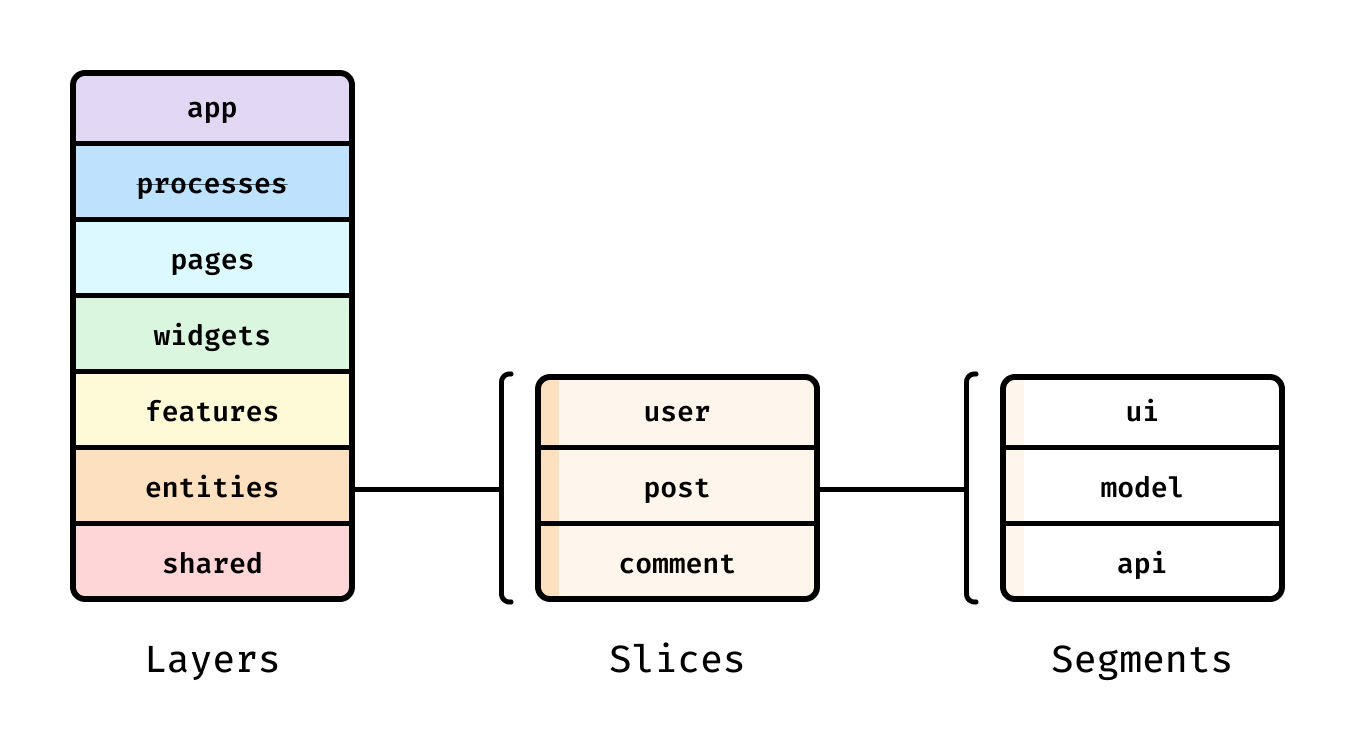
\includegraphics[width=0.7\linewidth]{static/fsdImage}
  \caption{Схема архитектуры клиентской части (FSD + Next.js)}
\end{figure}

На диаграмме представлены основные уровни и элементы архитектуры приложения. Следует отметить, что каждый слой в данной структуре ориентирован на строгое разграничение ответственности. Компоненты нижних уровней не имеют информации о вышестоящих слоях, что позволяет реализовать принцип инверсии зависимостей и минимизировать связанность между модулями.

\subsubsection{Слои архитектуры Feature-Sliced Design}

В таблице \ref{tab:fsd-layers} представлены слои архитектуры Feature-Sliced Design, сгруппированные по уровню абстракции и ответственности.

\begin{table}[h]
  \centering
  \caption{Слои архитектуры Feature-Sliced Design}
  \label{tab:fsd-layers}
  \begin{tabular}{|p{3cm}|p{11cm}|}
    \hline
    \textbf{Слой} & \textbf{Описание и назначение} \\ \hline
    \textit{app}      & Точка входа в приложение: глобальные стили, маршрутизация, провайдеры состояния, интеграции с внешними сервисами. \\ \hline
    \textit{pages}    & Страницы, связанные с маршрутизацией. Формируются из виджетов и не содержат бизнес-логики. \\ \hline
    \textit{widgets}  & Крупные элементы интерфейса, отражающие пользовательские сценарии, например, чат, список заданий, панель управления. \\ \hline
    \textit{features}& Изолированные пользовательские функции, такие как авторизация, отправка сообщений или регистрация. Могут включать бизнес-логику и вызовы API. \\ \hline
    \textit{entities} & Базовые предметные сущности предметной области, включающие типы, схемы, API и UI-представление. \\ \hline
    \textit{shared}   & Универсальные компоненты, утилиты и типы, переиспользуемые во всём проекте. \\ \hline
  \end{tabular}
\end{table}

\subsubsection{Концепция срезов (slices)}

Ключевым элементом архитектурного подхода Feature-Sliced Design является понятие срезов (англ. \textit{slices}). Под срезом понимается логически обособленный модуль, реализующий завершённую часть функциональности приложения. Каждый срез может содержать собственные модели данных, визуальные компоненты, бизнес-логику, а также механизмы взаимодействия с внешними источниками данных.

Например:
\begin{itemize}
  \item \textit{features/login} — срез, реализующий сценарий авторизации пользователя;
  \item \textit{entities/task} — срез, содержащий всё, что связано с сущностью «задание»;
  \item \textit{widgets/ChatWindow} — срез, объединяющий функциональность и интерфейс чат-интерфейса;
  \item \textit{pages/home} — срез, реализующий главную страницу приложения.
\end{itemize}

\subsubsection{Горизонтальное деление на сегменты (segments)}

Каждый срез, независимо от своего уровня, может быть дополнительно разделён на сегменты (англ. \textit{segments}) — логические подкатегории, структурирующие содержимое среза по назначению кода. В отличие от слоёв, которые представляют вертикальную иерархию, сегменты формируют горизонтальное деление и обеспечивают внутреннюю организацию модулей.

Наиболее распространённые типы сегментов включают:
\begin{itemize}
  \item \textit{ui} — визуальные компоненты и стили, определяющие отображение данных;
  \item \textit{model} — модели данных, хранилища состояния, типизация и бизнес-логика;
  \item \textit{api} — функции для работы с внешними сервисами, включая описание типов запросов и маппинг ответов;
  \item \textit{lib} — вспомогательные функции и библиотеки, используемые в пределах данного среза;
  \item \textit{config} — конфигурационные файлы и переключатели функциональности.
\end{itemize}

\subsubsection*{Преимущества выбранного подхода}

Применение архитектуры Feature-Sliced Design в контексте разрабатываемого клиентского приложения позволило достичь следующих результатов:
\begin{itemize}
  \item Чёткое разграничение обязанностей между модулями и слоями,
  \item Улучшенная масштабируемость проекта без деградации структуры,
  \item Повышенная модульность, обеспечивающая лёгкость в тестировании и повторном использовании кода,
  \item Создание условий для быстрой и эффективной интеграции новых членов команды в разработку,
  \item Архитектура, ориентированная на задачи и бизнес-логику, а не на технические детали.
\end{itemize}

В совокупности данные свойства делают архитектурное решение устойчивым к росту функциональности, улучшая поддержку и развитие системы в долгосрочной перспективе.
\subsection{Проектирование интерфейсных подсистем и экранов}

Одной из ключевых задач при проектировании клиентской части является логическое и функциональное разделение интерфейса на подсистемы, каждая из которых реализует отдельный аспект пользовательского взаимодействия. Такое разделение позволяет обеспечить модульность, переиспользуемость компонентов и устойчивость к изменениям.

Проект разрабатывается в архитектуре Feature-Sliced Design, что накладывает дополнительную дисциплину на организацию экранов и компонентов: все подсистемы формируются из \texttt{entities}, \texttt{features}, \texttt{widgets} и собираются в \texttt{pages}, а общая инфраструктура — в слое \texttt{shared}.

\subsubsection{Выделение ключевых интерфейсных подсистем}

Клиентская часть разработанной платформы организована в виде набора функционально обособленных интерфейсных подсистем, каждая из которых отвечает за определённый аспект пользовательского взаимодействия и бизнес-логики. Такое разграничение позволяет повысить масштабируемость и сопровождаемость системы, а также упростить процесс тестирования и внедрения новых функций.

На основании анализа требований к функциональности приложения и сценариев использования пользователями различных ролей (администратор, преподаватель, студент), были выделены следующие ключевые подсистемы.

\begin{enumerate}
  \item \textbf{Подсистема авторизации и регистрации}\\
  Отвечает за обеспечение безопасного входа в систему, регистрацию новых пользователей и управление сессиями. Аутентификация реализована с применением библиотеки \texttt{Auth.js} и технологии JSON Web Token (JWT), что позволяет надёжно разграничивать доступ к различным разделам интерфейса в зависимости от роли пользователя.  

  Регистрация в системе представлена в виде трёх пользовательских сценариев, адаптированных под особенности образовательного процесса:
  \begin{itemize}
    \item Первый сценарий реализован для новых организаций (институтов) и сопровождается созданием административной учётной записи. На этом этапе формируется корневая структура управления учреждением.
    \item Второй и третий сценарии предназначены для регистрации преподавателей и студентов соответственно. Оба сценария доступны исключительно по индивидуальным приглашениям, что обеспечивает контроль над составом участников образовательного процесса и предотвращает несанкционированный доступ.
  \end{itemize}
  
  Подсистема тесно связана с механизмами контроля прав доступа и маршрутизации, определяя поведение интерфейса в зависимости от текущего статуса пользователя.

  \item \textbf{Подсистема управления университетом}\\
  Реализует административную логику, связанную с конфигурацией организационной структуры образовательного учреждения (структура компонентов показана на Рис. \ref{fig:admin-components}).
  
  Основными функциями данной подсистемы являются:
  \begin{itemize}
    \item Создание и удаление структурных единиц — институтов, кафедр, учебных групп;
    \item Управление персоналом: добавление и блокировка преподавателей и студентов;
    \item Генерация приглашений для входа новых участников на платформу с конкретной ролью;
    \item Отображение данных по структуре учреждения.
  \end{itemize}
  
  Визуально подсистема представлена в виде панели управления с множеством таблиц, форм и интерактивных элементов, обеспечивающих быстрый доступ к ключевым административным операциям. Все действия защищены авторизацией и доступны только пользователям с соответствующими правами доступа.

  \item \textbf{Подсистема работы с заданиями и отправкой решений}\\
  Данная подсистема предназначена для организации учебной деятельности (структура компонентов представлена на Рис. \ref{fig:classroom-components}). 
  
  Основной интерфейс включает:
  \begin{itemize}
    \item Панель создания и редактирования заданий с параметрами проверки,
    \item Представление активных и завершённых заданий для студентов,
    \item Историю отправок с отображением результатов и статуса проверки.
  \end{itemize}
  
  Задания связаны с группами. Система также предоставляет базовую аналитику по результатам выполнения.

  \item \textbf{Подсистема обмена сообщениями (чаты)}\\ 
  В рамках образовательного процесса большое значение имеет возможность коммуникации (структура компонентов отображена на Рис. \ref{fig:chat-components}).
    
  \begin{figure}[H]
    \centering
    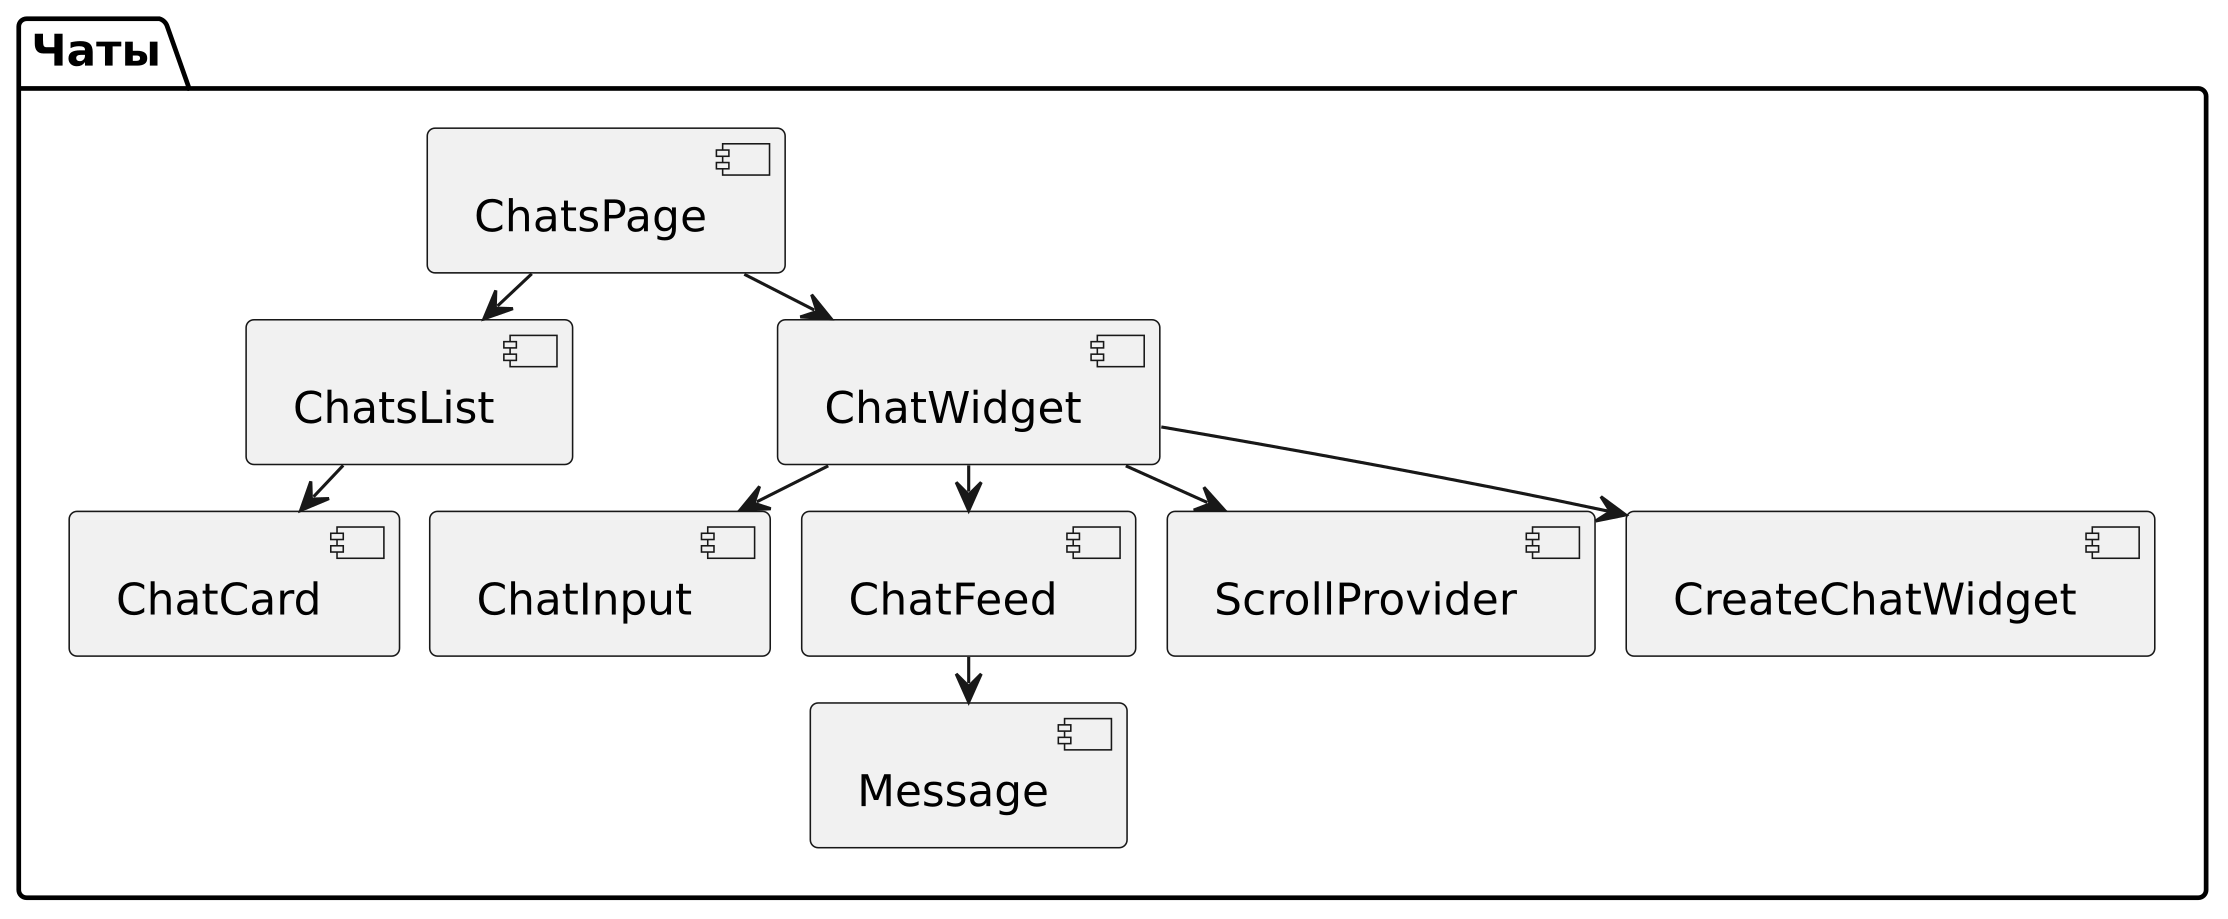
\includegraphics[width=0.9\textwidth]{static/diagrams/ChatsComponentDiagram.png}
    \caption{Диаграмма компонентов системы чатов}
    \label{fig:chat-components}
  \end{figure}
    
  Технически реализация основана на технологии WebSocket с использованием библиотеки \texttt{Socket.IO}, что обеспечивает мгновенную доставку сообщений и минимальную задержку при передаче данных.  
  
  Основной функционал включает:
  \begin{itemize}
    \item Подключение к соответствующим «комнатам» (группам или диалогам),
    \item Отправку и приём текстовых сообщений,
    \item Отображение истории переписки,
    \item Поддержку вложений и индикаторов прочтения.
  \end{itemize}
  
  Доступ к системе чатов осуществляется только после успешной авторизации, что исключает участие анонимных пользователей и обеспечивает безопасность переписки.

  \item \textbf{Подсистема AI-анализа решений}\\
  Одной из уникальных особенностей платформы является использование искусственного интеллекта для автоматической оценки студенческих заданий.
  
  Подсистема предназначена для получения и визуализации результатов AI-анализа, включающих:
  \begin{itemize}
    \item Оценку корректности кода;
    \item Проверку на соответствие заданию;
    \item Выявление потенциальных ошибок и некорректных конструкций;
    \item Комментарии, рекомендации и текстовые пояснения.
  \end{itemize}
  
  Результаты анализа отображаются в виде отчёта с возможностью преподавателя оставить дополнительные замечания. Таким образом, снижается нагрузка на преподавателя и повышается объективность оценивания.

\end{enumerate}

Каждая из указанных подсистем обладает чётко определёнными входными и выходными данными, а также взаимодействует с другими модулями системы. Например, подсистема работы с заданиями напрямую связана как с AI-анализом, так и с интерфейсами преподавателя и студента, а система чатов — с механизмами авторизации и маршрутизации. Такое проектирование обеспечивает гибкость, надёжность и чёткую масштабируемость клиентской архитектуры.

\subsubsection{Страницы и их структура}

Разработка интерфейсной части веб-приложения требует не только реализации функциональных компонентов, но и проектирования логически связанных экранов, отражающих ключевые сценарии взаимодействия пользователя с системой. В рамках платформы каждая страница представляет собой самостоятельный интерфейсный модуль, обслуживающий одну или несколько бизнес-задач, соответствующих определённой роли: студент, преподаватель, администратор.

Процесс формирования страниц реализован с применением маршрутизации, встроенной в фреймворк \texttt{Next.js}, что обеспечивает высокую производительность и поддержку серверного рендеринга. Страницы не только представляют визуальный уровень приложения, но и координируют работу между компонентами пользовательского интерфейса, бизнес-логикой и хранилищем состояния. 

Архитектурно страницы собираются из обособленных функциональных элементов, разработанных согласно принципам FSD: пользовательские действия реализуются в слое \texttt{features}, отображаемые сущности формируются на базе \texttt{entities}, а объединение этих блоков происходит внутри \texttt{widgets}. Такой подход позволяет повысить согласованность, переиспользуемость и модульность кода, а также снижает зависимость между различными частями интерфейса.

Ниже приведён перечень ключевых страниц, отражающих основную логику пользовательского взаимодействия.

\begin{itemize}
  \item \textbf{Страница авторизации}\\  
  Отвечает за вход пользователя в систему. Содержит форму для ввода учётных данных, а также реализует логику валидации, передачи данных на сервер, обработки ошибок и сохранения сессионного токена. После успешной авторизации пользователь перенаправляется на главную страницу, соответствующую его роли.

  \item \textbf{Страница заданий}\\
  Представляет собой ключевой интерфейс для организации и выполнения учебной деятельности. Интерфейс страницы включает:
  \begin{itemize}
    \item Список классов и учебных групп, к которым привязан пользователь,
    \item Перечень активных заданий в рамках каждой группы,
    \item Доступ к подробному описанию заданий, срокам сдачи и параметрам оценивания,
    \item Отправку решений и просмотр результатов, включая отчёты AI-анализа.
  \end{itemize}
  Для преподавателя дополнительно предоставляется интерфейс управления заданиями, а также доступа к аналитике по группам и студентам.

  \item \textbf{Административная панель института}\\
  Данная страница является основным рабочим инструментом пользователя с ролью администратора. Интерфейс включает:
  \begin{itemize}
    \item Управление иерархией образовательного учреждения (институты, кафедры, группы);
    \item Назначение и блокировка пользователей (студентов и преподавателей);
    \item Просмотр структуры учреждения в табличной форме;
    \item Генерацию и отправку приглашений на регистрацию;
    \item Журнал событий и контроль активности пользователей.
  \end{itemize}
  Все действия на данной странице требуют повышенного уровня доступа и сопровождаются системой уведомлений о результатах операций.

  \item \textbf{Страница чатов}\\
  Реализует коммуникационную составляющую платформы. Пользователь получает доступ к:
  \begin{itemize}
    \item Перечню активных диалогов (личных и групповых),
    \item Истории сообщений в рамках выбранного чата,
    \item Форме для отправки сообщений и файлов,
    \item Интерактивным элементам: индикаторы доставки, статус прочтения, поиск по переписке.
  \end{itemize}
  Для преподавателей также предусмотрена возможность создания новых групповых чатов для своих учебных групп.
\end{itemize}

Все функциональные страницы приложения, за исключением экранов регистрации и входа, используют единый шаблон компоновки \texttt{AppLayout}, обеспечивающий целостность визуального восприятия и унификацию пользовательского опыта. Данный шаблон включает в себя общие элементы интерфейса — верхнюю панель навигации, боковое меню и основной контейнер для отображения содержимого, который динамически наполняется в зависимости от текущего маршрута. 

Использование общего каркаса позволяет сохранить структурную согласованность между различными разделами системы, облегчает адаптацию пользователей к интерфейсу и упрощает внедрение изменений. Кроме того, архитектурное разделение логики и представления на уровне страниц способствует инкапсуляции ответственности, а также повышает читаемость и сопровождаемость кода. В рамках маршрутизации обеспечивается централизованное управление доступом, фильтрацией и визуализацией данных с учётом ролей пользователей.

Таким образом, структура страниц приложения отражает как технические требования архитектуры, так и практическую ориентацию на удобство и эффективность работы конечных пользователей.

\subsubsection{Компоненты и принципы их структурирования}

Компонентная модель проекта выстроена на основе принципов повторного использования, инкапсуляции и чёткого разделения ответственности между уровнями абстракции. Все компоненты, применяемые в рамках клиентского интерфейса, условно делятся на два основных класса: общие (универсальные) и специфические (бизнес-ориентированные).

\begin{itemize}
  \item \textbf{Общие компоненты} (\texttt{shared/ui}) представляют собой переиспользуемые элементы пользовательского интерфейса, не зависящие от предметной области. К ним относятся кнопки, поля ввода, модальные окна, индикаторы загрузки, элементы навигации, уведомления и другие базовые визуальные элементы. Такие компоненты широко применяются на всех уровнях интерфейса и не содержат бизнес-логики.
  
  \item \textbf{Специфические компоненты}, разрабатываемые в слоях \texttt{entities} и \texttt{widgets}, предназначены для реализации прикладной логики и отображения конкретных сущностей системы. Примерами являются компоненты отображения сообщений в чате, карточек заданий, панели управления преподавателя, таблиц пользователей и др. Они обладают внутренним состоянием и часто включают обращение к хранилищу или API.
\end{itemize}

Такое структурное разграничение существенно упрощает масштабирование проекта, облегчает поддержку и повторное использование элементов, а также способствует разделению труда между разработчиками.

\subsubsection{Распределение логики по слоям архитектуры}

Функциональная логика клиентской части системы строго распределяется по слоям архитектуры Feature-Sliced Design, что обеспечивает высокую модульность и инкапсуляцию поведения. Каждому слою соответствует свой уровень ответственности:

\begin{itemize}
  	\item В слое \texttt{entities} сосредоточена модель предметной области: типизация, структура сущностей, атомарные компоненты отображения, такие как \texttt{Registration}, \texttt{Department}, \texttt{Group}. Данный слой реализует описание и базовое представление данных без привязки к конкретным действиям пользователя.
  
	\item Слой \texttt{features} содержит реализацию отдельных действий, составляющих пользовательские сценарии: отправка сообщений, регистрация, загрузка задания, подтверждение действия и т.д. Эти модули инкапсулируют конкретные шаги взаимодействия пользователя с интерфейсом, часто включая локальное состояние и вызовы к API. \texttt{Features} могут быть использованы многократно и комбинироваться для построения более сложных сценариев.
	
	\item Слой \texttt{widgets} представляет собой реализацию полноценных пользовательских сценариев — законченных интерфейсных блоков, решающих определённую задачу. Примеры: интерфейс чата, панель с заданиями, административный модуль управления группами. Каждый виджет объединяет несколько фич и сущностей, обеспечивая завершённую и логически связанную единицу поведения.
	
	\item Слой \texttt{pages} выполняет роль точки входа и финальной сборки пользовательских сценариев. Здесь происходит выбор и компоновка виджетов в зависимости от маршрута, роли пользователя и контекста сессии. Кроме того, на уровне страниц задаются глобальные обёртки, обеспечиваются ограничения доступа, инициализируются загрузки данных и подключаются необходимые провайдеры. Таким образом, \texttt{pages} являются связующим слоем между навигацией и пользовательским опытом.
\end{itemize}

Такое строгое распределение обязанностей по слоям позволяет исключить дублирование логики, минимизировать связанность между модулями и обеспечить чёткую иерархию ответственности.

\subsubsection{UX-решения и пользовательские сценарии}

Для повышения удобства и доступности платформы, особенно в условиях использования её разными категориями пользователей, были реализованы следующие решения в области пользовательского опыта (UX):

\begin{itemize}
  \item \textbf{Централизованная навигация} — через универсальный макет, включающий боковую и верхнюю панели, интерфейс остаётся единообразным и интуитивно понятным вне зависимости от текущего маршрута.
  \item \textbf{Toast-уведомления} — реализация мгновенной обратной связи при выполнении действий: успешная отправка формы, ошибка сети, получение новых сообщений;
  \item \textbf{Обработка пустых состояний и ошибок} — предусмотрены интерфейсы для ситуаций отсутствия данных, ошибок загрузки или недоступности сервера.
\end{itemize}

В результате, пользователь получает предсказуемый и непрерывный опыт взаимодействия с системой вне зависимости от своей роли и уровня подготовки.

\subsubsection*{Вывод}

Проектирование интерфейсной части приложения основывается на чётком структурном и функциональном разграничении компонентов, ориентированном на принципы модульности и масштабируемости. Использование архитектуры Feature-Sliced Design позволяет изолировать бизнес-логику, визуальные компоненты и маршрутизацию, что делает интерфейс легко расширяемым и сопровождаемым.

Реализованная организация интерфейса, объединяющая единый шаблон компоновки, повторно используемые компоненты и специфические бизнес-модули, способствует формированию целостного пользовательского опыта. Выбранные UX-решения обеспечивают удобство и логичность навигации, а также высокую отзывчивость системы при взаимодействии с пользователем.


Интерфейсная часть проекта построена на модульной архитектуре, основанной на бизнес-функциях. Подсистемы выделены логически, а их реализация изолирована в независимые модули, что повышает удобство поддержки, расширения и переиспользования компонентов.
\subsection{Проектирование взаимодействия с сервером и WebSocket}

Клиентская часть приложения активно взаимодействует с сервером для получения и отправки данных, а также поддерживает постоянное соединение с помощью WebSocket в рамках подсистемы обмена сообщениями. При проектировании механизма взаимодействия были учтены требования безопасности, стабильности соединения, обработки ошибок, а также необходимость автоматического обновления сессионных данных пользователя.

\subsubsection{Аутентификация и управление токенами}
Для обеспечения защищённого доступа к функциональности платформы используется система авторизации с применением JSON Web Token (JWT). Управление сессией пользователя реализовано через библиотеку \texttt{Auth.js}, которая выполняет роль промежуточного слоя между клиентом и системой хранения токенов.

\begin{enumerate}
  \item \textbf{Аутентификация пользователя}:
  \begin{itemize}
    \item пользователь выполняет вход с помощью логина/пароля или через OAuth-провайдеров (например, Google);
    \item Auth.js инициирует процесс аутентификации и получает JWT при успешной проверке.
  \end{itemize}.
  
  \item \textbf{Работа с токеном}:
  \begin{itemize}
    \item полученный JWT содержит минимальный необходимый payload (например, идентификатор пользователя, роль и срок действия);
    \item токен сохраняется в \texttt{HTTP-only} cookie с флагами \texttt{Secure} и \texttt{SameSite=Strict}, что предотвращает XSS- и CSRF-атаки.
  \end{itemize}.
  
  \item \textbf{Доступ к защищённым ресурсам}:
  \begin{itemize}
    \item при обращении к API front-end автоматически прикрепляет токен к запросу;
    \item при недействительном или истёкшем токене Auth.js обновляет его через refresh-токен, если он присутствует.
  \end{itemize}.
\end{enumerate}

\subsubsection{Унифицированная функция отправки запросов}
Для стандартизации сетевого взаимодействия была разработана функция \texttt{sendRequest}, инкапсулирующая логику подготовки и отправки HTTP-запросов:
\begin{itemize}
  \item преобразование данных в JSON через \texttt{JSON.stringify};
  \item добавление заголовков, включая \texttt{Authorization: Bearer};
  \item обработка ошибок и повторная попытка после обновления токена;
  \item поддержка различных HTTP-методов.
\end{itemize}.

\subsubsection{Взаимодействие через WebSocket}
Для реализации обмена сообщениями в реальном времени используется библиотека \texttt{Socket.IO}, обеспечивающая:
\begin{itemize}
  \item автоматическое переподключение при обрыве соединения;
  \item передачу структурированных событий с именами и аргументами;
  \item интеграцию с middleware для авторизации;
  \item работу с пространствами имён и комнатами;
  \item fallback-транспорты при недоступности WebSocket.
\end{itemize}.

На стороне клиента реализован хук \texttt{useSocket}, который:
\begin{itemize}
  \item инициализирует соединение с сервером;
  \item отправляет и получает события с типизированными данными;
  \item подписывается и отписывается от каналов;
  \item управляет жизненным циклом подключения и логирует события;
  \item обрабатывает ошибки соединения.
\end{itemize}.

При установлении WebSocket-соединения клиент передаёт access-token в параметрах, сервер проверяет его и активирует соединение. В случае истечения срока действия токена:
\begin{enumerate}
  \item инициируется его обновление;
  \item текущее соединение закрывается;
  \item создаётся новое соединение с обновлённым токеном.
\end{enumerate}

\subsubsection*{Вывод}

Реализованные механизмы автоматического обновления токенов, единая функция отправки запросов и продуманная интеграция WebSocket через \texttt{Socket.IO} обеспечивают безопасность, надёжность и масштабируемость взаимодействия клиентской части с сервером в режиме реального времени.

\subsection{Интеграция ИИ-модуля DeepSeek в архитектуру проекта}

Для обеспечения эффективной работы ИИ-компонента в образовательной платформе реализована модульная архитектура с чётким разделением ответственности. Последующие подразделы детализируют ключевые аспекты интеграции: стратегию контейнеризации для изоляции сервиса, механизмы взаимодействия с клиентской частью и системные преимущества выбранного подхода. Основное внимание уделено сохранению прозрачности работы ИИ для конечных пользователей при обеспечении гибкости разработки и эксплуатации.

\subsubsection{Контейнеризация DeepSeek}
Для обеспечения независимого жизненного цикла и лёгкой масштабируемости ИИ-компонента DeepSeek развёртывается в виде изолированного Docker-контейнера. Такой подход позволяет:

\begin{itemize}
  \item быстро запускать и останавливать сервис без влияния на основное приложение;
  \item поддерживать разные версии DeepSeek параллельно, экспериментируя с обновлениями моделей;
  \item мигрировать между хостами и облачными средами с минимальными изменениями конфигурации.
\end{itemize}

\subsubsection{Преимущества контейнеризированного подхода}
Контейнеризация DeepSeek даёт следующие ключевые плюсы:
\begin{itemize}
  \item \textbf{Изоляция нагрузки}: анализ кода выполняется в отдельном окружении, не влияя на отзывчивость интерфейса;
  \item \textbf{Горизонтальное масштабирование}: при большом числе запросов можно запускать несколько инстансов контейнера;
  \item \textbf{Упрощённое сопровождение}: обновление ИИ-компонента сводится к выпуску нового Docker-образа без правок во фронтенде;
  \item \textbf{Гибкость развертывания}: контейнеры можно запускать локально и в облаке с одинаковой конфигурацией.
\end{itemize}

\subsubsection{Взаимодействие клиентской части с DeepSeek}

Клиентская часть приложения, реализованная на React и Next.js, отправляет HTTP-запросы к back-end части Web-приложения при прикреплении решения задания студентом, далее back-end автоматически начинает проверку решения при помощи AI-анализа. Результат проверки приходит пользователю при запросе на получения детальной информации по задаче, выполненной студентом.

\begin{figure}[H]
    \centering
    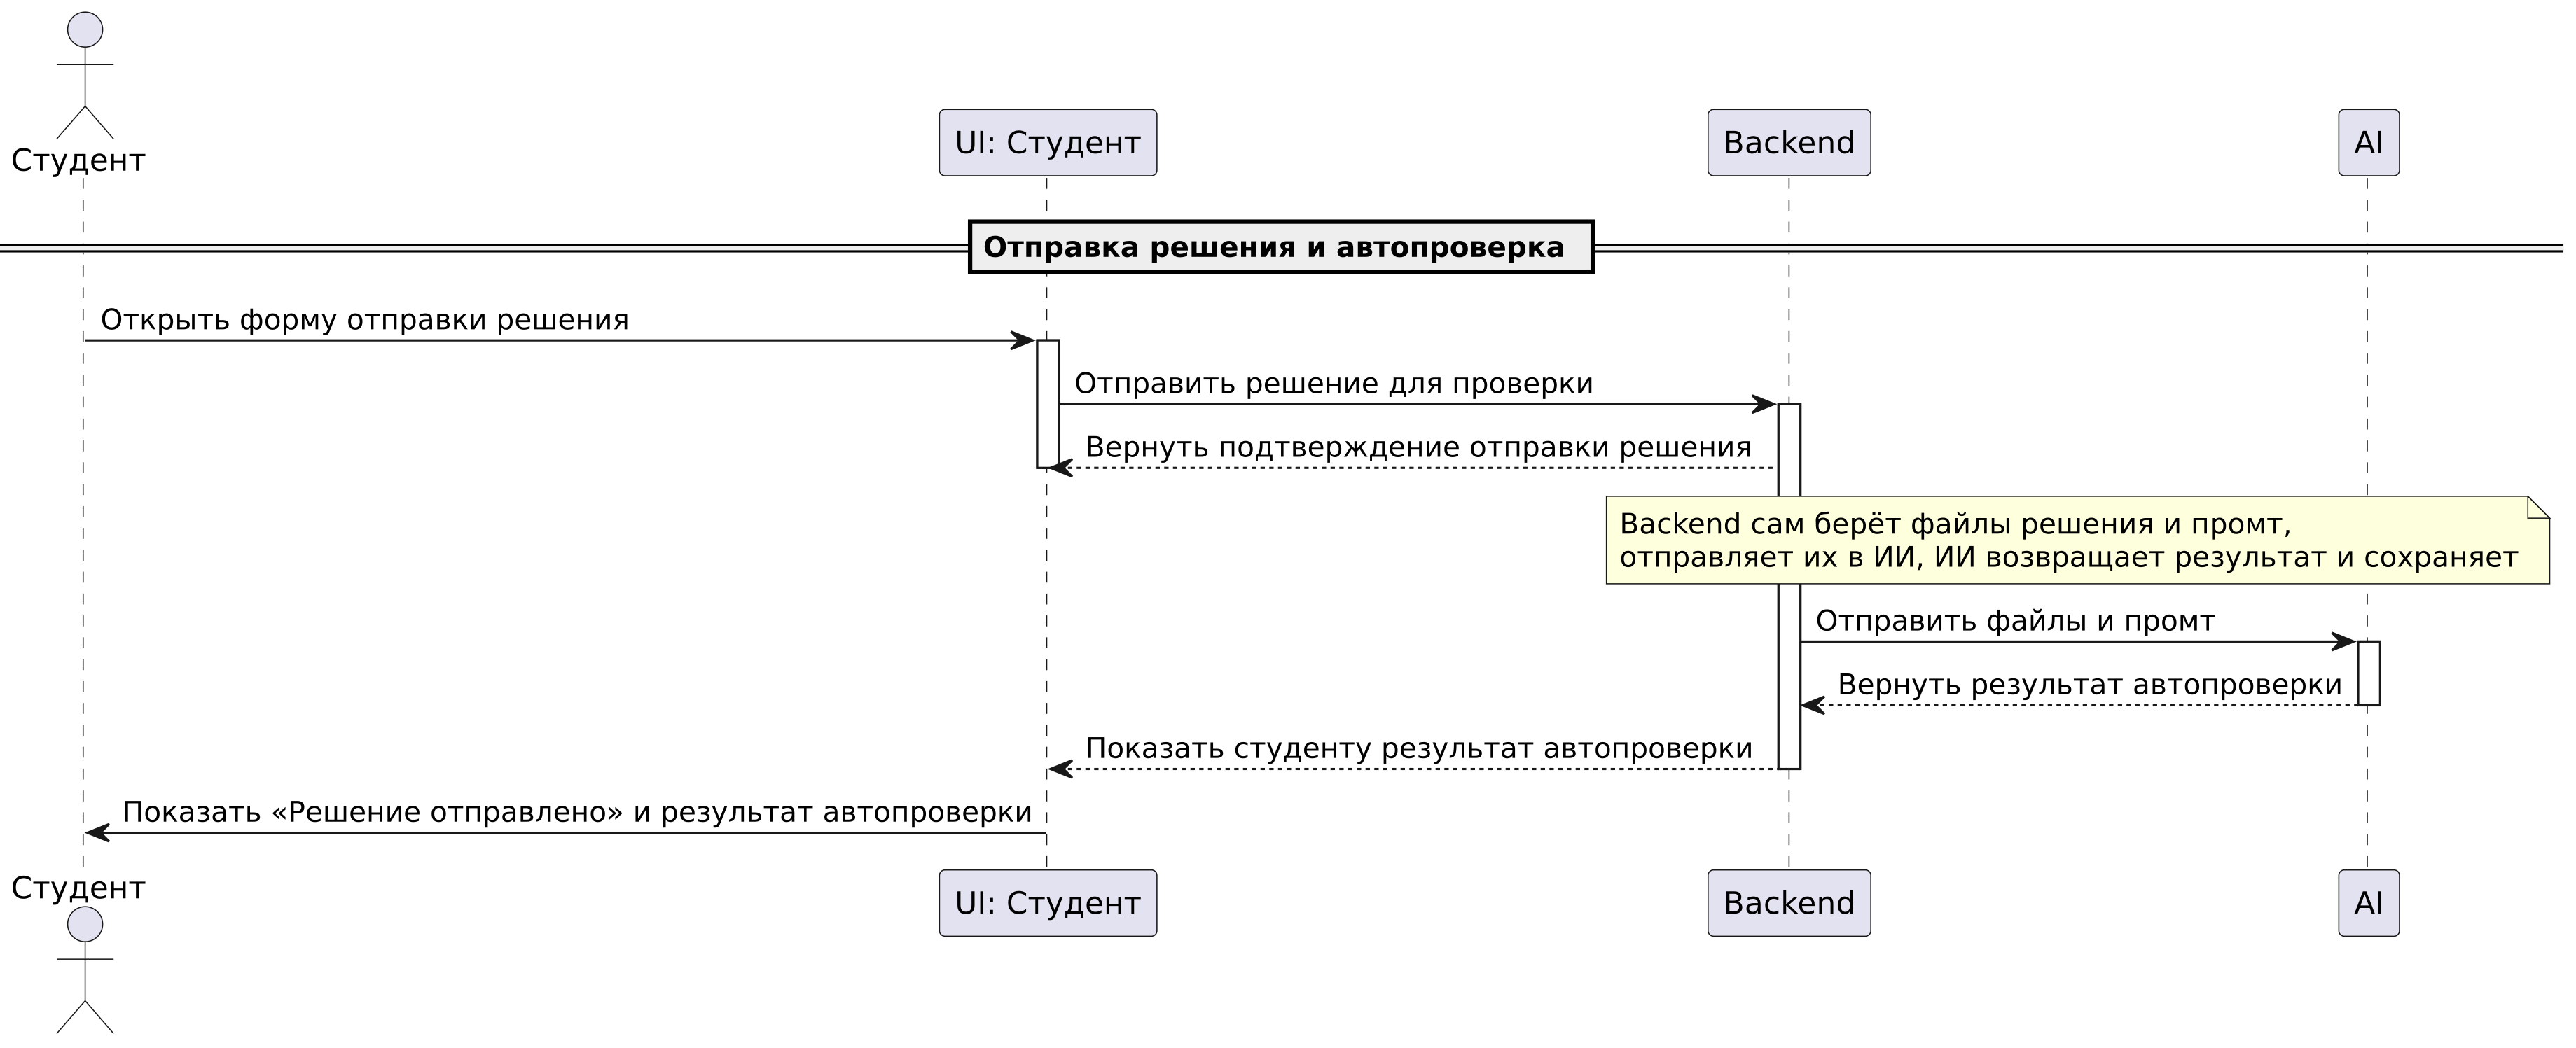
\includegraphics[width=0.8\linewidth]{static/diagrams/TaskSendStudentDiagram.png}
    \caption{Схема взаимодействия клиентской части (React/Next.js) с модулем DeepSeek}
    \label{fig:client-deepseek}
\end{figure}

На рисунке \ref{fig:client-deepseek} представлена схема взаимодействия клиентской части с модулем DeepSeek.

\subsubsection{Вывод}

Контейнеризация DeepSeek обеспечивает полную независимость остальных компонентов приложения от ИИ-модуля, позволяя развёртывать и обновлять его без влияния на другие сервисы. Взаимодействие через API бэкенда создаёт своего рода «чёрный ящик» для клиента, что упрощает инкапсуляцию логики и даёт гибкость в распределении и масштабировании нагрузки на контейнер с AI.



\subsection{Обеспечение безопасности клиентской части}

Безопасность пользовательского взаимодействия является важнейшей составляющей архитектуры клиентской части платформы. В условиях, когда доступ к различным модулям приложения осуществляется на основе ролей, а взаимодействие с данными сопровождается отображением пользовательского контента, особое внимание уделяется как управлению доступом, так и защите от потенциальных атак, включая межсайтовое выполнение скриптов (XSS). В данной подсистеме реализован комплекс механизмов, направленных на защиту данных и поведения интерфейса со стороны клиента.

\subsubsection{Разграничения доступа}
Одним из ключевых компонентов обеспечения безопасности клиентской части является система контроля доступа на основе промежуточного слоя — промежуточное программное обеспечение~\cite{nextjs_middleware}. В рамках архитектуры \textit{Next.js}, промежуточное программное обеспечение представляет собой функцию, исполняемую при каждом запросе к защищённым маршрутам. Она позволяет перехватывать обращения к страницам до их рендеринга и на этой стадии выполнять необходимые проверки: наличие токена, его валидность, а также права пользователя.

В контексте реализуемой платформы при обращении пользователя к любой защищённой странице клиентская логика через промежуточное программное обеспечение извлекает JWT-токен из cookies и дешифрует его содержимое, получая полезную нагрузку — уникальный идентификатор, срок действия сессии и роль в системе (\textit{admin}, \textit{teacher}, \textit{student}).

На основе этой информации промежуточное программное обеспечение выполняет следующие действия:
\begin{itemize}
  \item Если пользователь не авторизован (отсутствует валидный токен) — происходит автоматический редирект на страницу входа.
  \item Если пользователь авторизован, но не обладает достаточными правами — осуществляется перенаправление на главную страницу или отображается сообщение об отказе в доступе.
  \item Если пользователь обладает необходимой ролью — доступ к ресурсу предоставляется, и страница загружается с соответствующим контентом.
\end{itemize}

Таким образом, промежуточное программное обеспечение дает надёжную фильтрацию обращений к различным частям интерфейса, предотвращая несанкционированный доступ и соблюдая политику разграничения прав.

\subsubsection{Роль и защита при работе с форматируемым текстом}
Дополнительным вектором потенциальной угрозы в клиентских приложениях является отображение форматируемого текста, особенно если пользователь имеет возможность редактировать его содержимое. В таких случаях возрастает риск внедрения вредоносных скриптов, замаскированных под обычный HTML.

Для решения данной задачи в проекте используется библиотека \textit{tiptap} — расширяемый редактор форматированного текста на основе \textit{ProseMirror}. Одним из ключевых преимуществ \textit{tiptap} является контроль над тем, какие HTML-теги и атрибуты допускаются к отображению. Таким образом, даже если пользователь попытается вставить опасный код, редактор удалит такие элементы на этапе парсинга.

Технически это реализуется следующим образом:
\begin{itemize}
  \item при вводе содержимого редактор не сохраняет «сырые» HTML-строки, а формирует безопасное представление согласно заданным схемам;
  \item при рендеринге текста из базы или состояния редактор отображает только те элементы, которые были описаны как допустимые;
  \item расширения (extensions), добавляемые к \textit{tiptap}, позволяют точно контролировать список разрешённых тегов и атрибутов.
\end{itemize}

Таким образом, даже при наличии активной формы редактирования форматируемого текста пользовательская среда остаётся защищённой от внедрения опасного контента.

\subsubsection{Вывод}

Комплекс реализованных решений позволяет эффективно защитить клиентскую часть приложения как от внешнего вмешательства, так и от ошибочного доступа пользователей. Промежуточное программное обеспечение производит проверку сессии и прав доступа до загрузки страниц, а редактор \textit{tiptap} гарантирует безопасность при работе с форматируемым текстом. Такое сочетание архитектурных и прикладных средств создаёт устойчивую и безопасную пользовательскую среду.

\subsection{Покрытие бизнес-логики юнит-тестами}

Наш подход к обеспечению надёжности клиентского приложения фокусируется на обязательном юнит-тестировании бизнес-логики при помощи Jest. Тестирование UI-компонентов считается вторичным: написание и поддержка сравнений HTML-вывода часто оказывается более трудоёмким и хрупким, чем простая визуальная валидация. Визуальный осмотр интерфейса преподавателем или дизайнером даёт более быстрый и надёжный результат без лишних накладных расходов.

Основные принципы нашего подхода:
\begin{enumerate}
  \item Юнит-тесты покрывают функции, отвечающие за валидацию данных, расчёт оценок и другие критичные механизмы, гарантируя корректность работы независимо от изменений UI;
  \item Модульные тесты интерфейсов не используются: динамика верстки и частые мелкие правки приводят к избыточным провалам тестов и дополнительным усилиям на их поддержку;
  \item Благодаря отказу от snapshot-тестирования HTML структура текста программы остаётся гибкой, а команда освобождает время на развитие функциональности вместо постоянной правки тестов;
  \item Автоматический запуск тестов бизнес-логики при каждом пуше позволяет мгновенно обнаруживать регрессии и поддерживать стабильность продукта;
  \item Для окончательной валидации интерфейса используется ручной осмотр ключевых страниц после сборки, что даёт уверенность в корректности отображения без сложных технических средств.
\end{enumerate}

Такой подход обеспечивает надёжность самой логики приложения и упрощает работу с UI: вместо громоздких автоматизированных тестов на вёрстку мы применяем человеческую экспертизу для финальной проверки внешнего вида и пользовательского опыта.

\newpage
\ESKDthisStyle{formII}
\section{ПРОГРАММНАЯ РЕАЛИЗАЦИЯ}
\ESKDcolumnII{ПРОГРАММНАЯ РЕАЛИЗАЦИЯ}

\setcounter{figure}{0} 
\makeatletter
  \renewcommand{\thefigure}{3.\arabic{figure}}
\makeatother

\setcounter{table}{0}
\makeatletter
  \renewcommand{\thetable}{3.\arabic{table}}
\makeatother

\subsection{Архитектура по Feature-Sliced Design}

Feature-Sliced Design (FSD) — это гибкий набор рекомендаций и подходов по логической организации клиентского кода, основанных на выделении независимых функциональных слоёв и зон ответственности. В отличие от строгих стандартов, FSD предоставляет разработчикам свободу выбора конкретных решений, сохраняя при этом единый общий каркас структуры. Такая архитектура повышает читаемость, масштабируемость и тестируемость приложения, а также упрощает командную разработку и поддержку кода.

\subsubsection{Слой \textit{shared}}

Слой \textit{shared} служит хранилищем нижнего уровня для общих и переиспользуемых компонентов, утилит и ресурсов, не зависящих от конкретной бизнес-логики:
\begin{itemize}
  \item UI-компоненты общего назначения: простые React-компоненты (кнопки, лоадеры, таблицы, модальные окна), не содержащие бизнес-логику и используемые в различных контекстах;
  \item Провайдеры контекста: \textit{DragAndDropFilesProvider}, \textit{EnterKeyHandlerProvider} и другие, обеспечивающие единообразную работу с событиями и состояниями по всему приложению;
  \item Утилиты и хелперы: функции для форматирования дат и чисел, генерации уникальных идентификаторов, работы с \textit{localStorage} и пр.;
  \item Кастомные хуки общего назначения: \textit{useSearchParamsListener}, \textit{useWindowSize}, \textit{usePreviousValue} и другие, сокращающие дублирование кода;
  \item SVG-иконки и графика: импорт через SVGR для единообразного подключения и управления атрибутами SVG;
  \item Компоненты навигации и управления состоянием: \textit{PaginationComponent} для пагинации через URL-параметры, \textit{Breadcrumbs}, \textit{Tabs} и т. д.
\end{itemize}

\subsubsection{Слой \textit{entities}}

Слой \textit{entities} отвечает за интеграцию с внешними сервисами и описывает доменные модели:
\begin{itemize}
  \item \textit{api/}: тонкий слой-абстракция над HTTP-клиентами (\textit{fetch}/\textit{axios}), где функции названы в соответствии с операциями Swagger/OpenAPI (например, \textit{getUserProfile}, \textit{createOrder});
  \item \textit{types/}: TypeScript-интерфейсы и типы для запросов и ответов (например, \textit{UserProfileResponseType}, \textit{OrderCreateRequestBodyType});
  \item \textit{models/}: классы и mapper-функции для преобразования сырых данных из API в удобные объекты;
  \item \textit{services/}: обёртки для работы с локальным кэшем (IndexedDB, \textit{localStorage}) и реализации retry-логики и таймаутов.
\end{itemize}

\subsubsection{Слои \textit{features}, \textit{widgets}, \textit{pages}}

Главные рабочие слои приложения, отвечающие за реализацию конкретной функциональности:
\begin{enumerate}
  \item \textit{pages}: маршрутизация и верхний уровень страниц, описывающий пути, guards для доступа, асинхронную загрузку данных и выбор виджетов;
  \item \textit{widgets}: презентационные и «умные» компоненты по Smart/Presentational-паттерну:
    \begin{itemize}
        \item \emph{Presentational Component} — презентационный компонент, содержащий исключительно UI-логику и пропсы, без работы с API и глобальным состоянием;
        \item \emph{Smart Hook} — умный хук, содержащий всю бизнес-логику и передающий необходимые данные в презентационные компоненты.
    \end{itemize}
  \item \textit{features}: бизнес-логика и состояние в виде кастомных хуков, редьюсеров, слайсов Redux или Zustand:
    \begin{itemize}
      \item \textit{hooks.ts}: главный хук-фабрика (например, \textit{useRegistrationUniversity});
      \item \textit{schema.ts}: схемы форм;
      \item \textit{utils.ts}: вспомогательные функции и селекторы;
      \item \textit{store.ts}: подключение к Redux/Redux Toolkit.
    \end{itemize}
\end{enumerate}

\subsubsection{Пример виджета RegistrationUniversity}

В листинге~\ref{lst:registration-university-widget} представлен презентационный компонент, отвечающий за отображение формы регистрации университета.

\begin{lstlisting}[breaklines=true,caption=RegistrationUniversityWidget,label=lst:registration-university-widget]
  // Presentation-компонент
  export function RegistrationUniversityWidget() {
    const { formDataRef, isError, setIsError, onSubmit, isLoading } =
      useRegistrationUniversity();

    return (
      <div>...</div>
    );
  }
\end{lstlisting}

В листинге~\ref{lst:use-registration-university} представлен smart-hook, содержащий логику взаимодействия пользователя с формой регистрации университета и обработки отправки запроса на регистрацию.

\begin{lstlisting}[breaklines=true,caption=useRegistrationUniversity,label=lst:use-registration-university]
  // Smart-компонент: хук-фабрика
  export function useRegistrationUniversity() {
    const formDataRef = useRef<RegistrationData>();
    const [isError, setIsError] = useState<string[]>([]);
    const [isLoading, setIsLoading] = useState(false);
    const router = useRouter();

    const onSubmit = async () => {
      ...
    };
    return { formDataRef, isError, setIsError, onSubmit, isLoading };
  }
\end{lstlisting}

\subsubsection{Соглашения по именованию и структуре}

Для поддержания единого стиля и предсказуемости структуры проекта:
\begin{itemize}
  \item Имена функций API интерфейса и типов дублируют backend-операции;
  \item Компоненты и хуки получают префиксы по зоне ответственности (\textit{RegistrationForm}, \textit{useFilesUpload} и т. д.);
  \item В каждом каталоге \textit{features/FeatureName} обязателен минимум файлов: \textit{index.ts}, \textit{hooks.ts}, \textit{schema.ts}, \textit{utils.ts};
  \item Все слои описаны в README с диаграммой и примерами использования;
  \item Код-ревью включает проверку соответствия FSD-подходу и правилам TypeScript.
\end{itemize}

% Раздел 3.2: Собственная UI-библиотека и генерация форм
\subsection{Собственная UI-библиотека и генерация форм}

\subsubsection{Общая идея и мотивация}
Для обеспечения единого стилистического и функционального каркаса клиентского приложения была разработана собственная библиотека компонентов и утилит, распространяемая через npm-пакет. В её составе присутствуют:
\begin{enumerate}
  \item Набор готовых UI-компонентов (например, \textit{Button}, \textit{Tag}, \textit{ScrollProvider}), не содержащих бизнес-логику;
  \item Провайдеры глобальных состояний и контекстов (например, для управления скроллом или обработкой событий клавиатуры);
  \item Унифицированный генератор форм \textit{FormBuilder}, позволяющий описывать структуру и поведение сложных форм через декларативную схему.
\end{enumerate}
Применение данной библиотеки ускоряет процессы разработки и упрощает поддержку интерфейса, так как все ключевые решения собраны в централизованном модуле с единым API интерфейс и консистентной документацией.

\subsubsection{Компонент \textit{FormBuilder}}
Ключевым элементом библиотеки является компонент \textit{FormBuilder}. Он реализует маршрутизацию данных и событий между декларативной схемой формы и её полями. Основные принципы работы:
\begin{enumerate}
  \item Пользователь задаёт схему параметров формы, представляющую собой массив объектов с полем \textit{type} и соответствующим набором параметров;
  \item Компонент \textit{FormBuilder} инициализирует внутреннее состояние формы и передаёт каждому полю текущие значения и функции обработки изменений;
  \item При срабатывании события изменения значения поле уведомляет компонент \textit{FormBuilder}, который обновляет общую модель данных и вызывает функцию обратного вызова \textit{onChange}.
\end{enumerate}

Схема формы описывается функцией, возвращающей массив объектов. Каждый объект содержит \textit{type} — идентификатор типа элемента (например, \textit{input\_field} или \textit{array\_fields}), а также \textit{props} — набор свойств, необходимых для рендеринга и обработки (таких как имя поля, текст метки и дополнительные параметры). Пример описания схемы формы приведён в листинге~\ref{lst:form-scheme}.

\begin{lstlisting}[caption=Пример описания схемы формы,label=lst:form-scheme]
export function inviteTeacherScheme(): FORM_BUILDER_SCHEMA {
  return [
    {
      type: 'input_field',
      props: {
        name: 'email',
        labelText: 'Email'
      }
    },
    {
      type: 'input_field',
      props: {
        type: 'select',
        name: 'department_id',
        ownerInputComponent: <DepartmentSelectField />
      }
    }
  ];
}
\end{lstlisting}

Пример использования компонента \textit{FormBuilder} приведён в листинге~\ref{lst:formbuilder-usage}.

\begin{lstlisting}[caption=Использование \textit{FormBuilder},label=lst:formbuilder-usage]
<FormBuilder schema={inviteTeacherScheme()} 
			 onChange={onChangeFormData}/>
\end{lstlisting}

Компонент \textit{FormBuilder} автоматически распределяет данные между полями и собирает итоговый объект формы, передавая его через функцию \textit{onChange}.

\subsubsection{Типы элементов схемы и их поведение}
Ниже приведены ключевые типы схем, поддерживаемые компонентом \textit{FormBuilder}, и описание их функциональности.

Схема \textit{INPUT\_FIELD\_SCHEMA} отвечает за отображение и управление единичным полем ввода. Она включает обязательное поле \textit{name} (ключ в итоговом объекте данных), а также опциональные параметры: \textit{labelText} (отображаемая метка поля), \textit{hintText} (текст подсказки под полем), \textit{type} (уточнение типа поля, например \textit{select} или \textit{datetime}) и \textit{ownerInputComponent} (пользовательский компонент, принимающий параметры: \textit{value}, \textit{onChange}, \textit{isError} и \textit{onBlur}). Пример использования схемы представлен в листинге~\ref{lst:input-fields-schema}.

\begin{lstlisting}[caption={Пример INPUT\_FIELD\_SCHEMA},label={lst:input-fields-schema}]
const schema: INPUT_FIELD_SCHEMA = {
  type: 'input_field',
  props: {
    name: 'username',
    labelText: 'Имя пользователя',
    hintText: 'Введите ваш логин'
  }
};
\end{lstlisting}

Схема \textit{ARRAY\_FIELDS\_SCHEMA} предназначена для формирования массива однотипных входных полей, где все вложенные элементы \textit{input\_field} объединяются в массив. Обязательными параметрами схемы являются: \textit{name} (имя массива в итоговой модели данных) и \textit{children} (массив схем элементов, составляющих каждую отдельную запись). Пример использования данной схемы представлен в листинге~\ref{lst:array-fields-schema}.

\begin{lstlisting}[caption={Пример \textit{ARRAY\_FIELDS\_SCHEMA}},label={lst:array-fields-schema}]
const schema: ARRAY_FIELDS_SCHEMA = [
  {
    type: 'array_fields',
    props: {
      name: 'subjects',
      children: [
        {
          type: 'input_field',
          props: {
            name: 'subjectName',
            labelText: 'Название предмета'
          }
        }
      ]
    }
  }
];
\end{lstlisting}

Схема \textit{FORM\_WRAPPER\_SCHEMA} обеспечивает группировку полей без сброса индексов массивов, сохраняя вложенные элементы как объект. Обязательными параметрами выступают \textit{name} (ключ в результирующем объекте) и \textit{children} (схема вложенных элементов). Пример реализации приведён в листинге~\ref{lst:form-wrapper-schema}.

\begin{lstlisting}[caption={Пример \textit{FORM\_WRAPPER\_SCHEMA}},label={lst:form-wrapper-schema}]
const schema: FORM_WRAPPER_SCHEMA = [{
  type: 'form_wrapper',
  props: {
    name: 'teacherInfo',
    children: [
      {
        type: 'input_field',
        props: { name: 'firstName', labelText: 'Имя' }
      },
      {
        type: 'input_field',
        props: { name: 'lastName', labelText: 'Фамилия' }
      }
    ]
  }
}];
\end{lstlisting}

Схема \textit{BLOCK\_WRAPPER\_SCHEMA} позволяет визуально группировать элементы без изменения структуры данных: поля в нём обрабатываются как часть текущего массива или объекта. Пример схемы показан в листинге~\ref{lst:block-wrapper-schema}.

\begin{lstlisting}[caption={Пример \textit{BLOCK\_WRAPPER\_SCHEMA}},label={lst:block-wrapper-schema}]
const schema: BLOCK_WRAPPER_SCHEMA = [
  {
    type: 'block_wrapper',
    props: {
      children: [
        {
          type: 'input_field',
          props: {
            name: 'code',
            labelText: 'Код'
          }
        }
      ]
    }
  }
];
\end{lstlisting}

Схема \textit{REACT\_NODE\_SCHEMA} предназначена для вставки произвольного React-элемента в форму. Пример схемы показан в листинге~\ref{lst:react-node-schema}.

\begin{lstlisting}[caption={Пример \textit{REACT\_NODE\_SCHEMA}},label={lst:react-node-schema}]
const schema: REACT_NODE_SCHEMA = [
  {
    type: 'react_node',
    props: {
      node: <CustomSeparator />
    }
  }
];
\end{lstlisting}

\subsubsection{Преимущества и выводы}
Использование компонента \textit{FormBuilder} существенно снижает сложность создания многоуровневых форм:
\begin{enumerate}
  \item Единообразие описания различных полей;
  \item Возможность единообразной валидации и управления ошибками;
  \item Добавление новых полей сводится к регистрации нового блока схемы;
  \item Повышение читаемости текста программы: структура формы полностью отражена в схеме без дублирования логики в компонентах.
\end{enumerate}

% Конец раздела 3.2

\subsubsection{Работа с токеном JWT}
Для передачи и обновления JWT в сессии используется функция обратного вызова \textit{jwt}, принимающий параметр \textit{trigger}, позволяющий определить сценарий обработки. Логика работы примерно следующая: при первом входе пользователя (\textit{trigger = signIn}) в токен записываются поля \textit{access\_token}, \textit{refresh\_token} и прочие метаданные; при последующих запросах проверяется срок жизни \textit{access\_token}, и при необходимости инициируется процесс его обновления (\textit{trigger = update}). Если же токен ещё валиден, возвращается неизменённая структура. Пример реализации приведён в листинге~\ref{lst:jwt-callback}.

\begin{lstlisting}[caption={JWT-callback с учётом trigger}, label={lst:jwt-callback}]
	async jwt({ token, trigger, user, session }): Promise<JWT> {
		// Срабатывает при первичной аутентификации (signIn)
		if (trigger === 'signIn') {
			return { ...user, error: null };
		}
		// Если токена ещё нет (например, при восстановлении сессии из куки)
		if (token == null) {
			return { ...session?.user, error: 'another' } as JWT;
		}
		// При запросе обновления (trigger = 'update')
		if (trigger === 'update') {
			return await refreshingProcess(token);
		}
		// Во всех остальных случаях (токен валиден), возвращаем прежнее состояние
		return { ...token, error: null };
	},
\end{lstlisting}

Ниже на рисунке~\ref{fig:auth-refresh} показана вся последовательная диаграмма, иллюстрирующая проверку срока жизни JWT на клиенте и, при необходимости, получение нового JWT токена по токену обновления. Эта схема помогает понять, как именно библиотека Auth.js (или NextAuth.js) взаимодействует с сервером для устойчивого хранения и своевременного обновления токенов без лишних повторных запросов.

\begin{figure}[h]
    \centering
    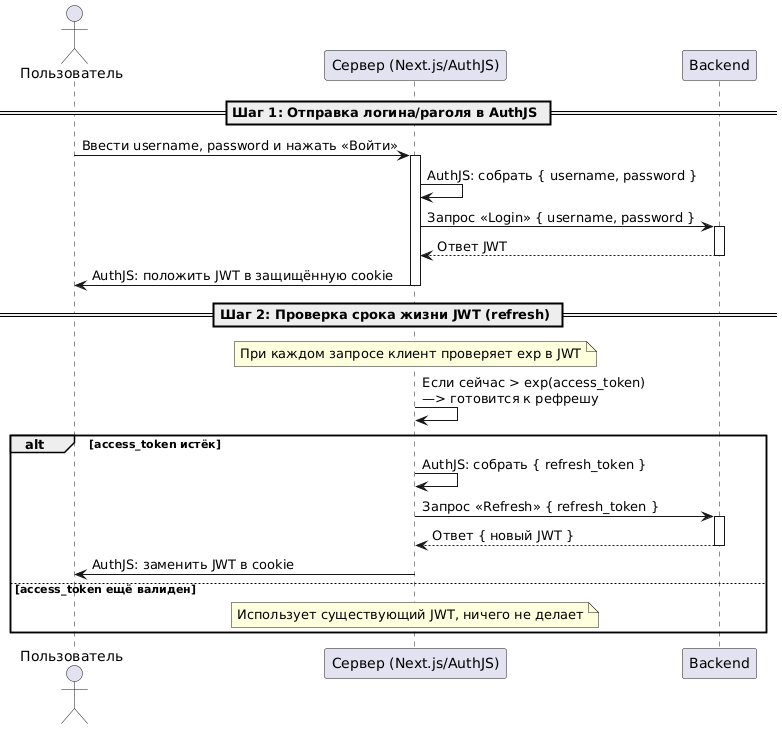
\includegraphics[width=0.9\textwidth]{static/diagrams/AuthRefresh.png}
    \caption{Схема процесса проверки и обновления JWT токена через токен обновления}
    \label{fig:auth-refresh}
\end{figure}

На рисунке~\ref{fig:auth-refresh} можно выделить два основных этапа: аутентификация пользователя и процесс использования токена.

При входе пользователя в систему происходит следующая последовательность действий:
\begin{enumerate}
    \item Пользователь вводит поля \textit{username} и \textit{password} в приложение;
    \item Модуль Auth.js формирует объект с учётными данными и отправляет запрос на сервер (метод \textit{login});
    \item Сервер возвращает токен доступа и токен обновления;
    \item Модуль Auth.js сохраняет полученный JWT в защищённую cookie или в хранилище клиента.
\end{enumerate}

После успешной аутентификации при каждом запросе выполняется проверка срока жизни токена и, при необходимости, его обновление.  Ниже приведены основные этапы этой проверки и процесса обновления::
\begin{enumerate}
    \item При каждом запросе клиент проверяет поле \textit{exp} (срок жизни) в токене доступа.
    \item Если текущий момент времени превысил время жизни токена доступа, начинается подготовка к обновлению токена.
    \item В случае истечения срока действия токена доступа модуль Auth.js отправляет токен обновления на сервер. Сервер возвращает новый токен доступа и новый токен обновления. После этого Auth.js заменяет старый токен в cookie браузера на новый.
    \item Если же токен доступа ещё валиден, Auth.js просто использует существующий токен и не делает дополнительных запросов (промежуточные уведомления внизу диаграммы).
\end{enumerate}

Таким образом, схема на рисунке~\ref{fig:auth-refresh} демонстрирует, что клиент всегда сначала пробует воспользоваться существующим токеном доступа, проверяя его валидность. Только если проверка не проходит, выполняется последовательность обновления, благодаря чему повышается отказоустойчивость и исключается ситуация «гонки» при параллельных запросах на обновление.

Важным дополнением к этой концепции является механизм предотвращения <<гонки состояний>> при одновременном запросе нескольких API-методов, обнаруживающих, что токен доступа просрочен. В таких случаях на клиенте сохраняется единственный промис обновления, который переиспользуется всеми последующими запросами до получения ответа от сервера. Пример реализации этого механизма приведён в листинге~\ref{lst:race-condition}.

\begin{lstlisting}[caption={Механизм предотвращения race condition при рефреше токена}, label={lst:race-condition}]
	export type RefreshPromiseStateType = Promise<JWT | null> | null;
	let tokenPromiseState: RefreshPromiseStateType = null;
	export const setTokenPromiseState = (
		promise: RefreshPromiseStateType
	): void => {
		tokenPromiseState = promise;
	};
	export const getTokenPromiseState = (): RefreshPromiseStateType => {
		return tokenPromiseState;
	};

	let tokenState: JWT | null = null;
	export const setTokenState = (newTokenState: JWT | null): void => {
		tokenState = newTokenState;
	};
	export const getTokenState = (): JWT | null => {
		return tokenState;
	};

	let timeoutState: NodeJS.Timeout | null = null;
\end{lstlisting}

На основе приведённой логики обеспечивается централизованная обработка авторизации и обновления токенов без дублирования текста программмы в разных частях приложения. Кроме того, использование одной общей очереди запросов к серверу для обновления JWT токена предотвращает нежелательные состояния гонки и лишние обращения к серверу.

% Раздел 3.4: Модуль «Регистрация и вход"
\subsection{Модуль «Регистрация и вход»}
В системе предусмотрены три сценария регистрации: для университета, студентов и преподавателей. В URL-параметрах \texttt{invite\_id} передаются данные приглашения для последующей валидации и передачи на бэкенд.

% Выбор виджета регистрации по типу
\begin{lstlisting}[caption={Выбор виджета регистрации}]
const getForm = () => {
    const type = getSearchParams(REGISTRATION_TYPE_PARAM_NAME) as RegistrationTypesType;
    const inviteId = getInviteId();
    switch (type) {
        case 'teacher':
            return <RegistrationTeacherWidget inviteId={inviteId} />;
        case 'student':
            return <RegistrationStudentWidget inviteId={inviteId} />;
        case 'university':
        default:
            return <RegistrationUniversityWidget />;
    }
};
\end{lstlisting}

Далее \texttt{invite\_id} передаётся в соответствующий виджет, который запрашивает на сервере данные приглашения. В случае неверного или просроченного ID отображается сообщение об ошибке.

% Виджет регистрации преподавателя
\begin{lstlisting}[caption={RegistrationTeacherWidget}]
export function RegistrationTeacherWidget({ inviteId }: RegistrationPropsType) {
    const { initData, onSubmit, isError, setIsError, formDataRef } =
        useRegistrationStudentAndTeacher<typeof registerTeacher>({
            inviteId,
            registrationRequest: registerTeacher
        });

    if (initData === undefined) {
        return 'Loading';
    }

    if (initData === null) {
        // Неверное приглашение или оно истекло
        return 'Error';
    }

	...
}
\end{lstlisting}

% Конец раздела 3.4

\subsubsection{Модуль формирования и отправки приглашений}
В административной панели университета реализован отдельный модуль, который позволяет формировать и отправлять приглашения как для преподавателей, так и для студентов. Этот модуль работает по следующему сценарию:

\begin{enumerate}
    \item \textbf{Инициация приглашения:} 
    \begin{itemize}
        \item администратор вводит в UI адрес электронной почты и идентификатор кафедры (для приглашения преподавателя) либо адрес электронной почты и идентификатор группы (для приглашения студента),
        \item после заполнения необходимых полей администратор нажимает кнопку «Сформировать ссылку».
    \end{itemize}
    \item \textbf{Отправка запроса на бэкенд:} 
    \begin{itemize}
        \item UI передаёт запрос на бэкенд, например, «Запрос на приглашение преподавателя (требуются: email, department\_id)» или «Запрос на приглашение студента (требуются: email, group\_id)»,
        \item бэкенд проверяет права администратора и корректность введённых данных, генерирует уникальную ссылку приглашения и возвращает её обратно в UI.
    \end{itemize}
    \item \textbf{Получение ответа и отображение ссылки:} 
    \begin{itemize}
        \item UI получает от бэкенда объект с полем \texttt{invite\_link},
        \item UI отображает администратору уведомление «Приглашение отправлено» и показывает полученную ссылку, которую можно скопировать и отправить по электронной почте.
    \end{itemize}
\end{enumerate}

На рисунке~\ref{fig:admin-invite} приведена последовательная диаграмма, иллюстрирующая полный процесс формирования и отправки приглашений: в верхней части — сценарий для преподавателя, в нижней части — сценарий для студента.

\begin{figure}[H]
    \centering
    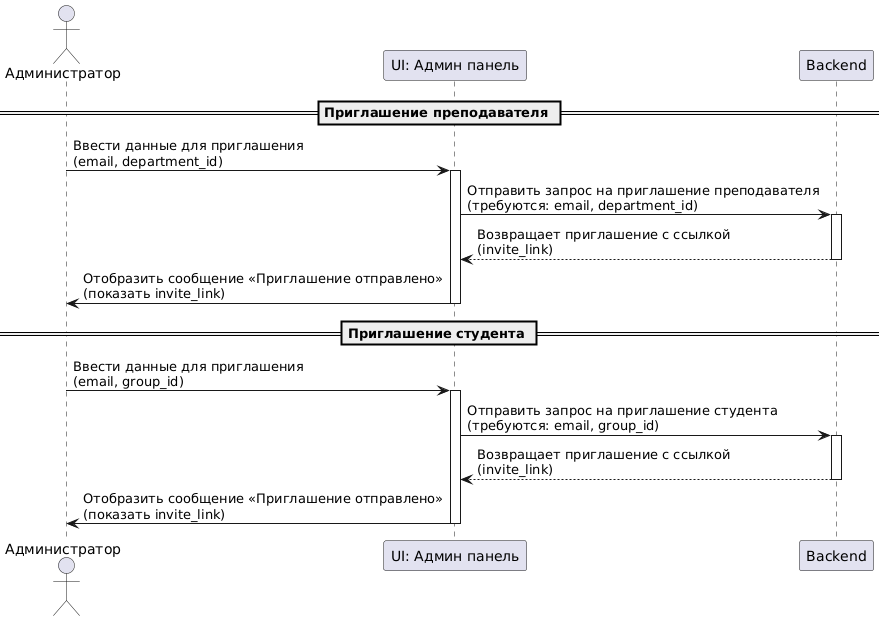
\includegraphics[width=0.9\textwidth]{static/diagrams/Admin.png}
    \caption{Схема процесса формирования и отправки приглашений преподавателям и студентам}
    \label{fig:admin-invite}
\end{figure}

На рисунке~\ref{fig:admin-invite} можно выделить следующие ключевые этапы:
\begin{itemize}
    \item \textbf{Приглашение преподавателя:}
    \begin{enumerate}
        \item администратор вводит в UI email и \texttt{department\_id},
        \item UI отправляет запрос на бэкенд «Приглашение преподавателя (требуются: email, department\_id)»,
        \item бэкенд проверяет данные, создаёт приглашение и возвращает уникальную ссылку (\texttt{invite\_link}),
        \item UI отображает сообщение «Приглашение отправлено» и показывает \texttt{invite\_link}.
    \end{enumerate}
    \item \textbf{Приглашение студента:}
    \begin{enumerate}
        \item администратор вводит в UI email и \texttt{group\_id},
        \item UI отправляет запрос на бэкенд «Приглашение студента (требуются: email, group\_id)»,
        \item бэкенд проверяет данные, создаёт приглашение и возвращает уникальную ссылку (\texttt{invite\_link}),
        \item UI отображает сообщение «Приглашение отправлено» и показывает \texttt{invite\_link}.
    \end{enumerate}
\end{itemize}

Таким образом, схема на рисунке~\ref{fig:admin-invite} демонстрирует единый алгоритм работы модуля: ввод данных в UI, отправка запроса на бэкенд, генерация и возврат уникальной ссылки, отображение ссылки администратору.

\subsubsection{Последовательная диаграмма работы модуля Classrooms}
Ниже приведена последовательная диаграмма, иллюстрирующая полный жизненный цикл взаимодействия преподавателя, студента, UI, бэкенда и AI-сервиса при работе с виртуальными классами и заданиями. На рисунке~\ref{fig:classroom-flow} показаны все основные этапы: создание класса, создание задания с указанием промта для автопроверки, получение списков заданий студентом, отправка решения студентом, автоматическая проверка через AI и выставление оценки преподавателем.

На рисунке~\ref{fig:classroom-flow} можно выделить следующие ключевые этапы:

\begin{enumerate}
    \item \textbf{Преподаватель создаёт класс:}
    \begin{itemize}
        \item преподаватель открывает форму создания класса в своем интерфейсе (UI: Преподаватель),
        \item UI отправляет запрос на бэкенд с данными нового класса,
        \item бэкенд возвращает подтверждение успешного создания (например, ID нового класса),
        \item UI отображает преподавателю сообщение «Класс создан».
    \end{itemize}

    \item \textbf{Преподаватель создаёт задание с возможностью задать промт для AI-проверки:}
    \begin{itemize}
        \item преподаватель переходит в форму создания задания, указывая вместе с условием текста задания промт для AI-проверки,
        \item UI отправляет запрос на бэкенд с данными задания и промтом,
        \item бэкенд возвращает подтверждение успешного сохранения задания,
        \item UI отображает преподавателю сообщение «Задание создано».
    \end{itemize}

    \item \textbf{Студент получает список доступных заданий:}
    \begin{itemize}
        \item студент открывает интерфейс (UI: Студент) и запрашивает список заданий для конкретного класса,
        \item UI отправляет запрос на бэкенд с ID класса,
        \item бэкенд возвращает массив доступных заданий,
        \item UI отображает студенту список заданий.
    \end{itemize}

    \item \textbf{Студент отправляет решение на проверку:}
    \begin{itemize}
        \item студент открывает форму отправки решения, выбирая конкретное задание,
        \item UI отправляет файлы решения и метаданные (например, ID задания, ID студента) на бэкенд,
        \item бэкенд возвращает подтверждение успешной загрузки решения,
        \item UI отображает студенту сообщение «Решение отправлено».
    \end{itemize}

    \item \textbf{Автопроверка через AI:}
    \begin{itemize}
        \item бэкенд получает файлы решения и ранее заданный промт к заданию,
        \item бэкенд отправляет файлы и промт во внешний AI-сервис,
        \item AI-сервис выполняет анализ кода (например, проверку корректности, стилевых нарушений и т. д.) и возвращает результат вместе с комментариями,
        \item бэкенд сохраняет результат автопроверки и передаёт его UI обоим ролям:
        \begin{enumerate}
            \item UI Студента: отображается результат автопроверки (оценка AI, комментарии),
            \item UI Преподавателя: отображается результат автопроверки (для последующей ручной проверки и выставления итоговой оценки).
        \end{enumerate}
    \end{itemize}

    \item \textbf{Преподаватель ставит оценку, и студент получает её:}
    \begin{itemize}
        \item преподаватель открывает форму выставления оценки (UI: Преподаватель) для конкретного решения,
        \item UI отправляет в бэкенд оценку и комментарий преподавателя,
        \item бэкенд сохраняет оценку, возвращает подтверждение сохранения,
        \item UI отображает преподавателю сообщение «Оценка сохранена», а UI Студента — обновлённую финальную оценку.
    \end{itemize}
\end{enumerate}

Таким образом, последовательная диаграмма на рисунке~\ref{fig:classroom-flow} демонстрирует весь цикл взаимодействий: от создания класса и задания преподавателем до получения студентом финальной оценки после автопроверки и ручного выставления оценки преподавателем.

\subsection{Модуль «Chats»}

\subsection{Тестирование}

В ходе разработки были протестированы модули как основного приложения, так и используемой при разработке библиотеки.

\subsubsection{Покрытие кода в приложении}

\begin{table}[h]
  \centering
    \small
  \caption{Покрытие кода клиентской части приложения.}
  \label{tab:app-coverage}
  \begin{tabular}{lrrrr}
  	\toprule
  	\textbf{File}                & \textbf{\%Stmts} & \textbf{\%Branch} & \textbf{\%Funcs} & \textbf{\%Lines} \\ \midrule
  	All files                    &            95.65 &             77.77 &           100.00 &           100.00 \\
  	features/Chats/lib           &           100.00 &            100.00 &           100.00 &           100.00 \\
  	\quad mergeMessages.ts       &           100.00 &            100.00 &           100.00 &           100.00 \\
  	shared/ui/TextEditor/lib     &            90.47 &             68.42 &           100.00 &           100.00 \\
  	\quad processTextToTiptap.ts &            94.11 &             72.22 &           100.00 &           100.00 \\
  	\quad processTiptapToText.ts &            75.00 &              0.00 &           100.00 &           100.00 \\ \bottomrule
  \end{tabular}
\end{table}

\noindent
В таблице~\ref{tab:app-coverage} приведены четыре основные метрики покрытия:
\begin{itemize}
  \item \%Stmts (Statements) — процент операторов кода, выполненных в ходе тестов;
  \item \%Branch (Branches) — процент ветвей условных операторов, затронутых тестами;
  \item \%Funcs (Functions) — процент функций, вызванных хотя бы одним тестом;
  \item \%Lines (Lines) — процент строк кода, исполненных тестами.
\end{itemize}
Для ключевых модулей (например, \textit{mergeMessages.ts}) все метрики равны 100\,\%.

\subsubsection{Покрытие кода в отдельной библиотеке}

\begin{table}[h]
  \small
  \centering
  \caption{Покрытие кода библиотеки компонентов.}
  \label{tab:lib-coverage}
  \begin{tabular}{lrrrr}
  	\toprule
  	\textbf{File}                           & \textbf{\%Stmts} & \textbf{\%Branch} & \textbf{\%Funcs} & \textbf{\%Lines} \\ \midrule
  	All files                               &            52.89 &             48.76 &            20.68 &            52.65 \\
  	lib/dict/getDeepValue.ts                &            86.36 &             73.33 &           100.00 &            85.71 \\
  	lib/dict/setDeepValue.ts                &           100.00 &            100.00 &           100.00 &           100.00 \\
  	ui/DateTimePicker/lib/changeInterval.ts &           100.00 &             96.29 &           100.00 &           100.00 \\ \bottomrule
  \end{tabular}
\end{table}

\noindent
В таблице~\ref{tab:lib-coverage} показано, что основные утилитные функции библиотеки (\textit{getDeepValue}, \textit{setDeepValue}, \textit{changeInterval}) полностью или почти полностью покрыты.

\subsubsection{Методы тестирования}

\begin{itemize}
  \item Модульное тестирование (unit testing):
    для каждой функции и компонента написаны независимые тесты, покрывающие:
    граничные и некорректные входные данные (undefined, пустые массивы), типичные сценарии и пограничные случаи.
  \item TDD–подход (Test–Driven Development):
    реализация функций по циклу «\textit{test → fail} → написать минимальный код → \textit{test → pass} → рефакторинг».
  \item Покрытие ветвлений (branch coverage):
    каждый сценарий условных операторов (\textit{if/else}, тернарные выражения, \textit{switch}) проверяется отдельными тестами.
  \item Round-trip-тесты:
    для преобразований «текст → HTML → текст» (функции \textit{processTextToTiptap} / \textit{processTiptapToText}) проверяется обратимость и корректность в сложных случаях (вложенные теги, переносы строк).
  \item Инструментация и сбор покрытия:
    запуск командой \textit{npx jest --coverage} автоматически оборачивает счётчиками все исходники и собирает метрики Statements, Branches, Functions и Lines.
\end{itemize}

\newpage
\ESKDthisStyle{formII}
\section*{ЗАКЛЮЧЕНИЕ}
\ESKDcolumnII{ЗАКЛЮЧЕНИЕ}

В рамках проведённой дипломной работы была спроектирована и реализована клиентская часть веб-приложения для управления образовательным процессом в университете. Основная цель заключалась в создании масштабируемой и легко расширяемой архитектуры интерфейса, обеспечивающей высокую консистентность, читаемость и удобство поддержки. С этой целью были выполнены следующие ключевые мероприятия:

\begin{itemize}
  \item 
  Исследован и успешно применён модульный подход, позволивший чётко разделить проект на уровни ответственности и упростить навигацию по коду.

  \item 
  Разработана собственная библиотека пользовательского интерфейса, включающая набор визуальных компонентов и механизм автоматической генерации форм на основе декларативных описаний. Эта библиотека обеспечила единообразие стилистики и сократила время на создание новых интерфейсных элементов.

  \item 
  Внедрена система аутентификации и авторизации с поддержкой долгосрочных сессий, способная автоматически обновлять токены доступа без вмешательства пользователя и обеспечивать надёжную защиту маршрутов с учётом разных типов пользователей.

  \item 
  Реализован универсальный механизм регистрации для различных ролей участников (администрации университета, преподавателей и студентов), включающий проверку приглашений и гибкую обработку ошибок серверной части.

  \item 
  Создана административная панель с возможностями просмотра, создания, редактирования и удаления данных университета, включая управление структурой институтов, кафедр и учебных групп. Интерфейс обеспечил интуитивный доступ к основным операциям благодаря адаптированным формам и табличным представлениям.

  \item 
  Построен модуль виртуальных классов, обеспечивающий создание и организацию учебных групп, назначение заданий и сбор обратной связи. Интеграция автоматизированного анализа решений студентов с использованием AI-технологий позволила существенно повысить качество проверки кода лабораторных работ.

  \item 
  Разработана система мгновенного обмена сообщениями в реальном времени, включающая надёжное WebSocket-соединение, устойчивое к временным сбоям сети, а также удобные механизмы загрузки истории переписки в обе стороны и оптимистичного обновления интерфейса при отправке новых сообщений.
\end{itemize}

Проведённая работа подтверждает достижение поставленных задач: предложенные архитектурные решения обеспечили гибкость и расширяемость, а использование современных технологий и инструментов ускорило реализацию функционала и повысило устойчивость системы. 

С практической точки зрения, клиентское приложение демонстрирует следующие преимущества:
\begin{itemize}
  \item Повышенная скорость разработки за счёт переиспользования компонентов и генерации форм;
  \item Улучшенная безопасность благодаря продуманной схеме управления сессиями и авторизацией;
  \item Удобство сопровождения за счёт модульности и чёткого разделения ответственности;
  \item Расширяемость и поддержка новых сценариев благодаря гибкому подходу к конфигурации интерфейса.
\end{itemize}

В дальнейшем целесообразно рассмотреть следующие направления развития:
\begin{itemize}
  \item Расширение возможностей автоматизированного анализа решений с учётом различных языков программирования и более глубокой семантической проверки;
  \item Добавление функционала офлайн-режима с последующей синхронизацией изменений;
  \item Разработку мобильных клиентских приложений для повышения доступности и удобства работы на мобильных устройствах;
  \item Внедрение системы аналитики и мониторинга пользовательской активности для оптимизации интерфейса и оценки эффективности процессов обучения.
\end{itemize}

Подведённые итоги свидетельствуют о высокой эффективности предложенного подхода и открывают перспективы дальнейших исследований и развития системы.

\ESKDthisStyle{formII}
\section*{СПИСОК ЛИТЕРАТУРЫ}
\addcontentsline{toc}{section}{СПИСОК ЛИТЕРАТУРЫ}
\ESKDcolumnII{СПИСОК ЛИТЕРАТУРЫ}
\vspace{-1.5\baselineskip}

\begingroup
  % Отключаем разрыв страницы перед/внутри и после thebibliography
  \let\clearpage\relax
  \let\newpage\relax
  % Переопределяем addcontentsline так, чтобы «съедать» все 3 аргумента
    \renewcommand{\addcontentsline}[3]{}
  % Подавляем автоматический заголовок, который thebibliography может вставлять
  \renewcommand{\refname}{}

  \begin{thebibliography}{99}

    \bibitem{1}
    TypeScript Handbook. Официальная документация. URL: \url{https://www.typescriptlang.org/docs/handbook/intro.html}.
    
    \bibitem{2}
    React. Официальная документация. URL: \url{https://reactjs.org/}.

    \bibitem{3}
    Next.js. Официальная документация. URL: \url{https://nextjs.org/docs}.

    \bibitem{4}
    Socket.IO. Официальная документация. URL: \url{https://socket.io/docs/}.

    \bibitem{5}
    Auth.js (ранее NextAuth.js). Официальная документация. URL: \url{https://next-auth.js.org/}.

    \bibitem{6}
    JSON Web Token (JWT). RFC 7519. URL: \url{https://tools.ietf.org/html/rfc7519}.

    \bibitem{7}
    MDN Web Docs. HTML. URL: \url{https://developer.mozilla.org/ru/docs/Web/HTML}.

    \bibitem{8}
    MDN Web Docs. CSS. URL: \url{https://developer.mozilla.org/ru/docs/Web/CSS}.

    \bibitem{9}
    MDN Web Docs. JavaScript. URL: \url{https://developer.mozilla.org/ru/docs/Web/JavaScript}.

    \bibitem{10}
    Habr. «SPA: преимущества и недостатки одностраничных приложений». URL: \url{https://habr.com/ru/post/451234/}.

    \bibitem{11}
    Habr. «SSR vs SSG в Next.js: что выбрать?» URL: \url{https://habr.com/ru/post/559876/}.

    \bibitem{12}
    Habr. «Современные фичи React 18 и их применение». URL: \url{https://habr.com/ru/post/568123/}.

    \bibitem{13}
    Habr. «Feature-Sliced Design: организация структуры Frontend-проекта». URL: \url{https://habr.com/ru/post/481567/}.

    \bibitem{14}
    Habr. «Управление состоянием в React с помощью Redux Toolkit». URL: \url{https://habr.com/ru/post/512345/}.

    \bibitem{15}
    Habr. «Лёгкие альтернативы Redux: обзор Zustand». URL: \url{https://habr.com/ru/post/537890/}.

    \bibitem{16}
    Habr. «Введение в WebSocket: что это и как работает». URL: \url{https://habr.com/ru/post/445678/}.

    \bibitem{17}
    Habr. «Авторизация и аутентификация в Next.js с Auth.js». URL: \url{https://habr.com/ru/post/583210/}.

    \bibitem{18}
    Habr. «Безопасность веб-приложений: защита JWT и CSRF». URL: \url{https://habr.com/ru/post/579432/}.

    \bibitem{19}
    Habr. «SCSS-препроцессор: основы и лучшие практики». URL: \url{https://habr.com/ru/post/520123/}.

    \bibitem{20}
    Habr. «Интеграция искусственного интеллекта в веб-приложение на примере Next.js». URL: \url{https://habr.com/ru/post/590456/}.

  \end{thebibliography}
\endgroup



\newpage

\ESKDthisStyle{formII}
\ESKDcolumnII{ПРИЛОЖЕНИЕ A}
\section*{ПРИЛОЖЕНИЕ A}
\addcontentsline{toc}{section}{ПРИЛОЖЕНИЕ A}

\setcounter{figure}{0} 
\makeatletter
  \renewcommand{\thefigure}{A.\arabic{figure}}
\makeatother


\begin{figure}[H]
\centering
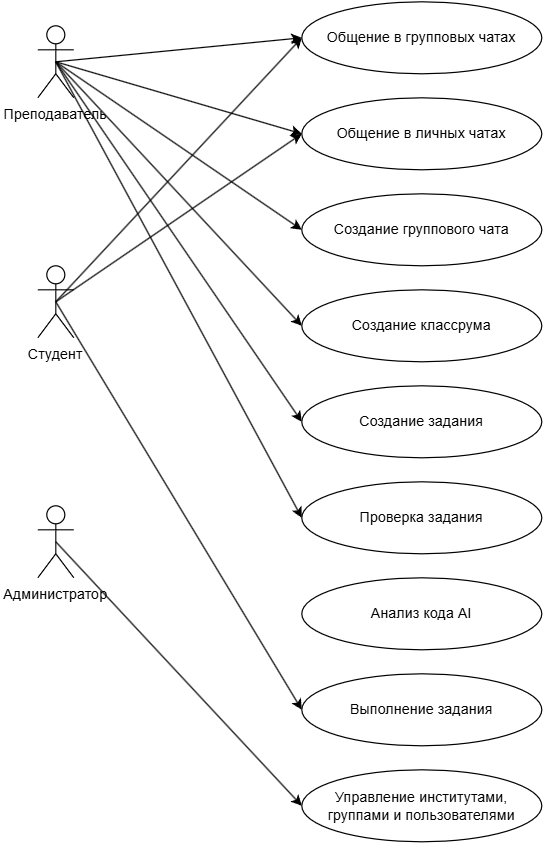
\includegraphics[width=0.5\linewidth]{static/useCaseDiagramm}
\caption{Диаграмма вариантов использования системы для различных ролей пользователей.}
\label{fig:usecasediagramm}
\end{figure}

\begin{figure}[H]
    \centering
    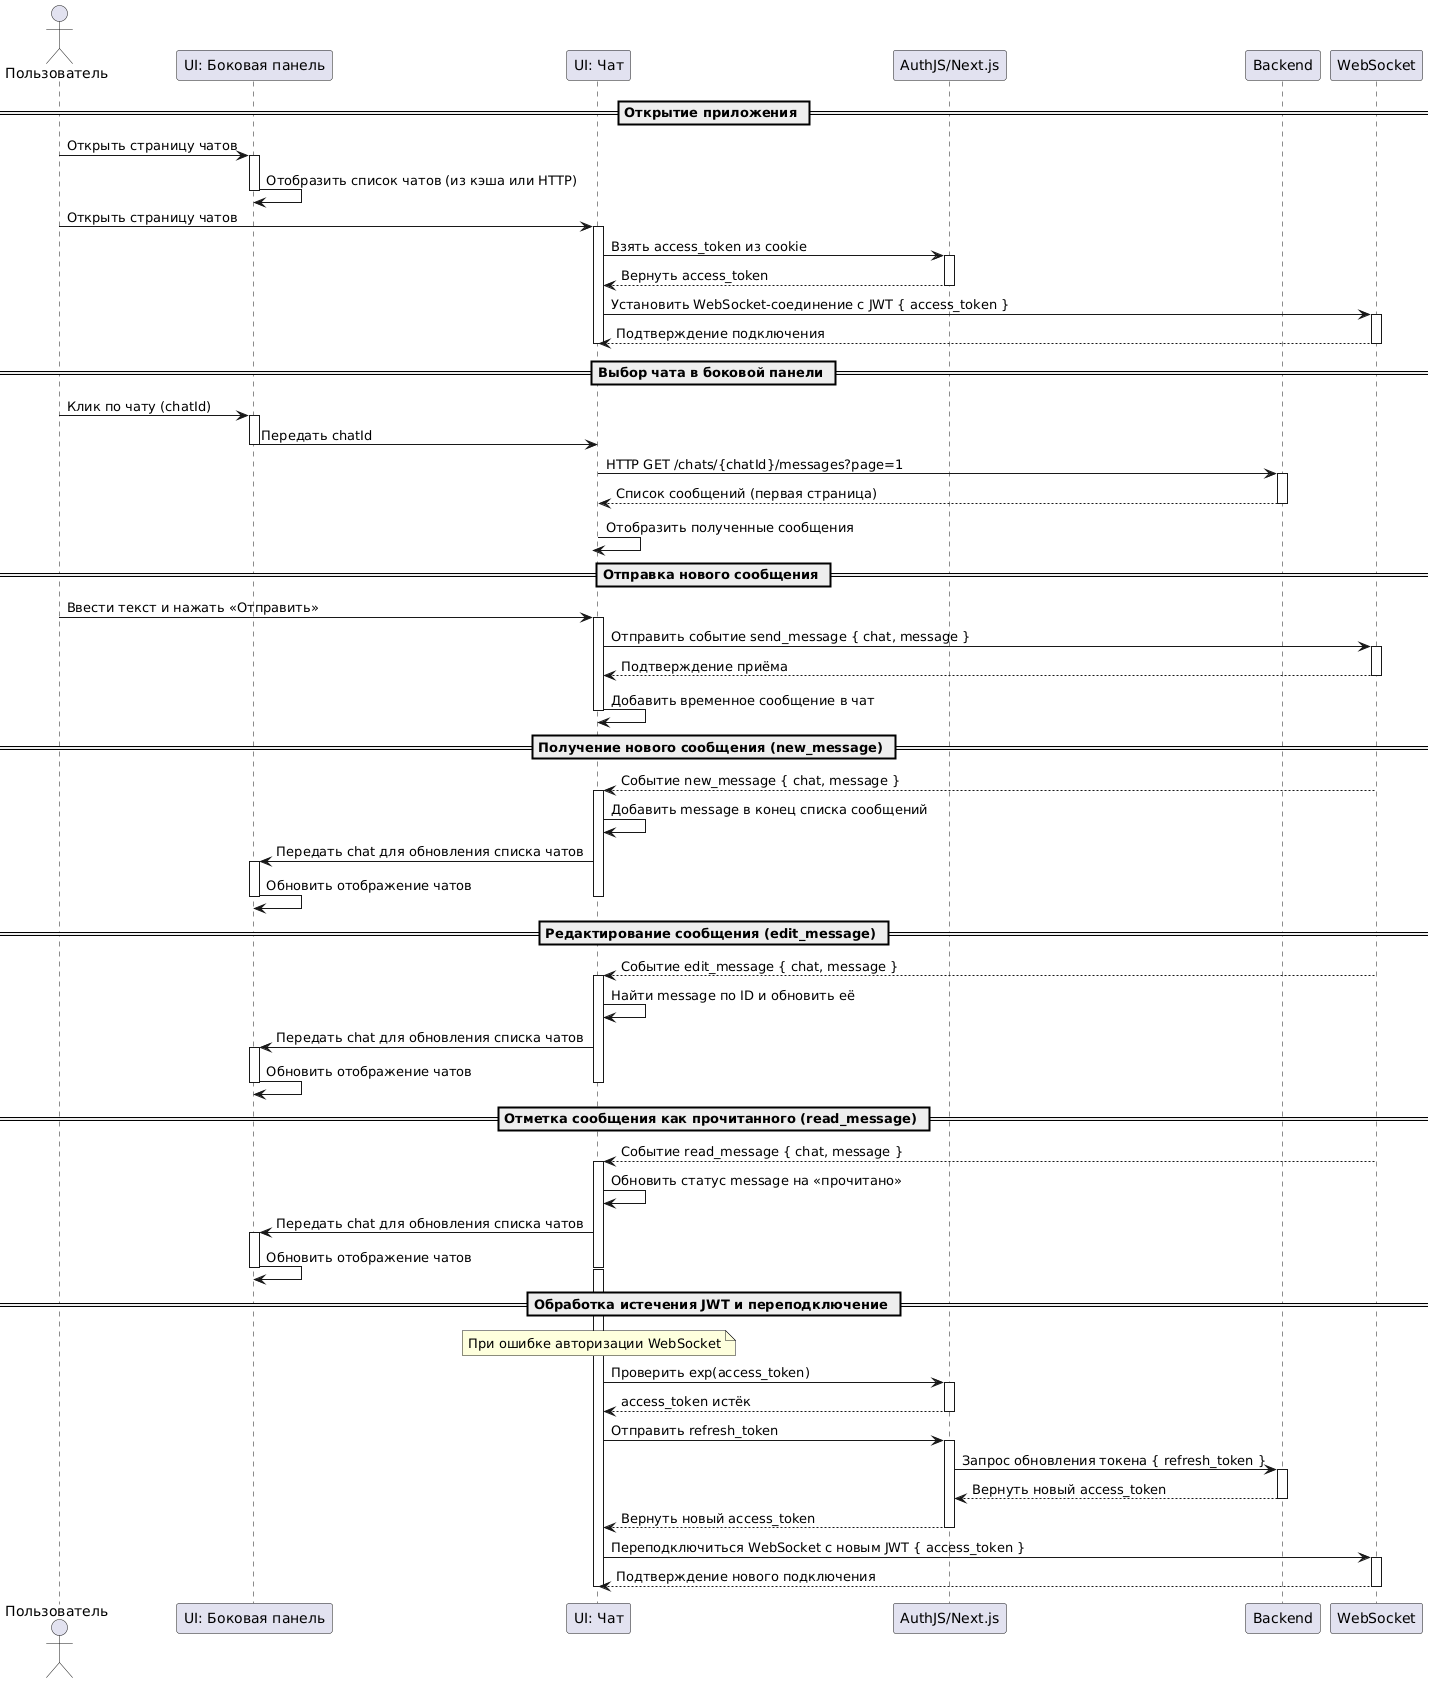
\includegraphics[width=0.9\textwidth]{static/diagrams/Chats.png}
    \caption{Схема взаимодействия клиента (UI: Боковая панель и UI: Чат), AuthJS (Next.js), бэкенда и WebSocket при работе модуля «Chats».}
    \label{fig:chats-flow}
\end{figure}


\begin{figure}[H]
    \centering
    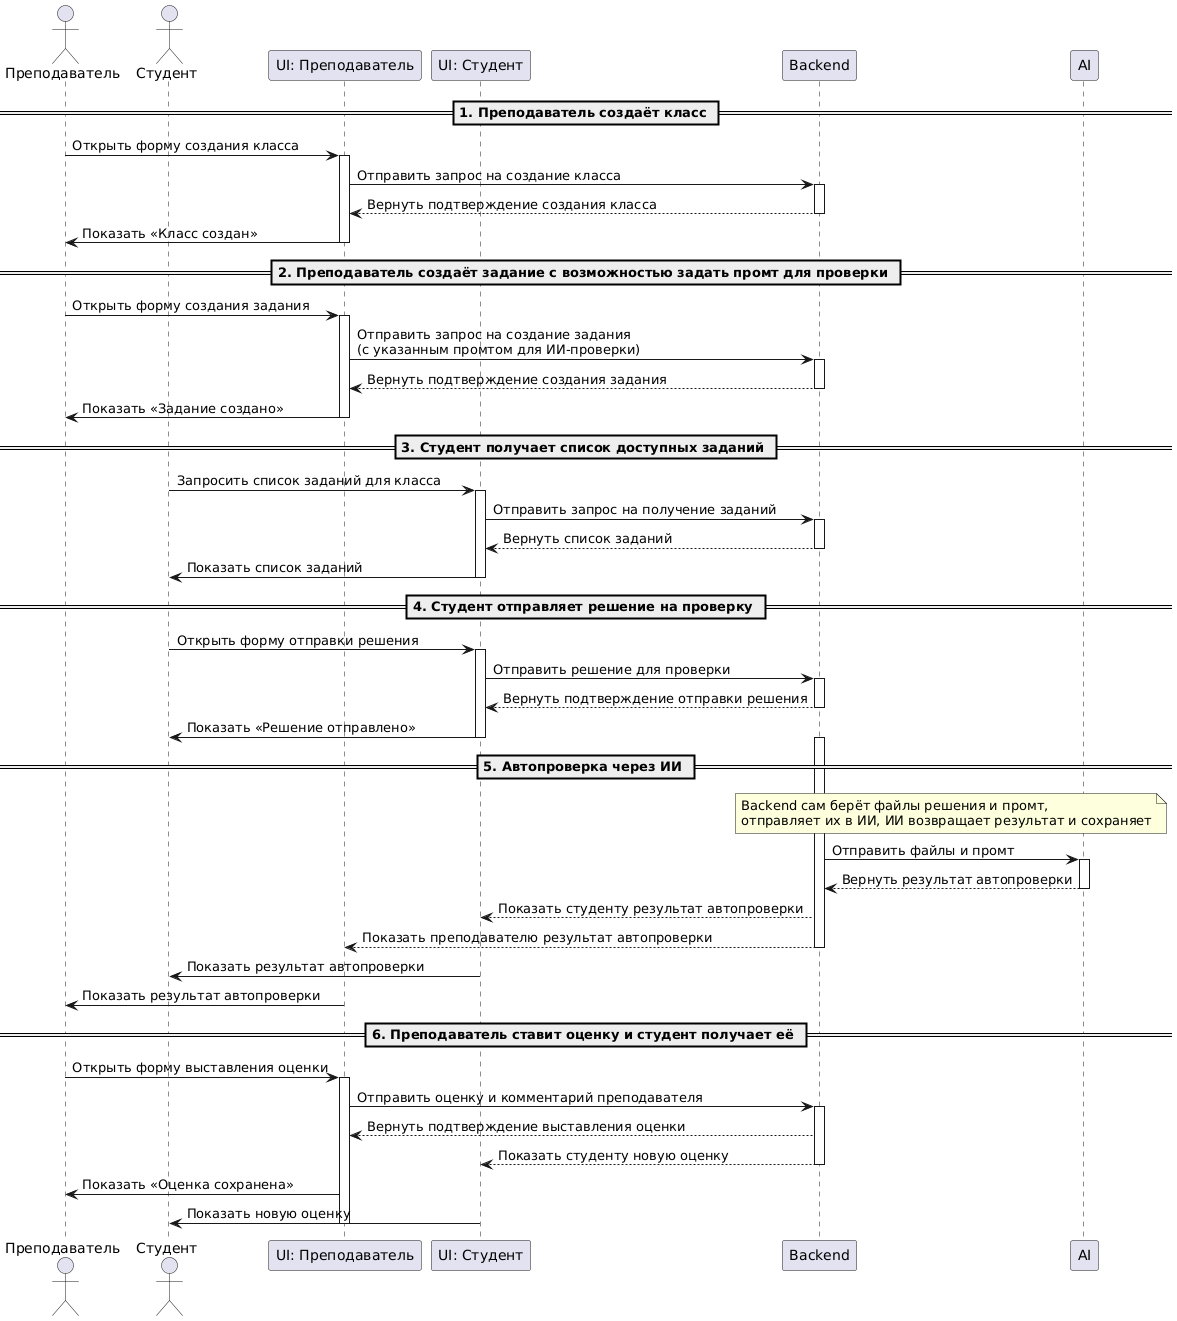
\includegraphics[width=0.9\textwidth]{static/diagrams/Classroom.png}
    \caption{Схема взаимодействия преподавателя, студента, UI, бэкенда и AI при работе с виртуальными классами}
    \label{fig:classroom-flow}
\end{figure}

\ESKDthisStyle{formII}
\ESKDcolumnII{ПРИЛОЖЕНИЕ Б}
\section*{ПРИЛОЖЕНИЕ Б}
\addcontentsline{toc}{section}{ПРИЛОЖЕНИЕ Б}

Исходный код фронтенда доступен в GitHub-репозитории:
\href{https://github.com/BeSmileV/unichat-front}{https://github.com/BeSmileV/unichat-front}

\end{document}
